\def\year{2016}\relax
%File: formatting-instruction.tex
\documentclass[letterpaper]{article}
\usepackage{aaai16}
\usepackage{times}
\usepackage{helvet}
\usepackage{courier}

\usepackage{graphicx}
\usepackage{epstopdf}
\usepackage[noend]{algorithmic}
\usepackage{algorithm}
\usepackage{amsmath}
\usepackage{amsfonts}


\frenchspacing
\setlength{\pdfpagewidth}{8.5in}
\setlength{\pdfpageheight}{11in}

\usepackage{amsmath,amssymb}
\newtheorem{theorem}{Theorem}
\newtheorem{lemma}{Lemma}
\newtheorem{corollary}{Corollary}
\newtheorem{example}{Example}
\newtheorem{definition}{Definition}
\newenvironment{proof}{\par\noindent{\em Proof.}}{\hfill $\Box$\medskip}
\def\minimize{\mathop{\mbox{\bf minimize}}}
\def\maximize{\mathop{\mbox{\bf maximize}}}
\def\subjectto{\mathop{\mbox{\bf subject to}}}
\DeclareMathOperator*{\argmin}{\arg\!\min}
\DeclareMathOperator*{\argmax}{\arg\!\max}
\newcommand{\GHS}{\mbox{\tt GHS}}
\newcommand{\CS}{\mbox{\tt CS}}
\newcommand{\roni}[1]{\mbox{\tt RONI: #1}}
\renewcommand{\algorithmicrequire}{\textbf{Input:}}
\renewcommand{\algorithmicensure}{\textbf{Output:}}


\pdfinfo{
/Title (Searching with a Corrupted Heuristic)
/Author (Put All Your Authors Here, Separated by Commas)}
\setcounter{secnumdepth}{0}  
 \begin{document}
% The file aaai.sty is the style file for AAAI Press 
% proceedings, working notes, and technical reports.
%
\title{Searching with a Corrupted Heuristic}
\author{Submission \#14}
\maketitle
\begin{abstract}
Memory-based heuristics are a popular and effective type of admissible heuristic functions. 
However, corruptions to memory may cause them to be inadmissible. Such corruptions can be caused, for example, by the physical environment in which the search algorithm is used such as radiation and network errors in case of a distributed memory. 
Error correcting codes can be used to limit the amount of corruption but at the cost of additional memory consumption. 
We introduce an error correction schemes that do not require additional memory and exploits knowledge about the behavior of admissible heuristic functions. 
Search algorithms using our methods are bounded-suboptimal and are guaranteed to find a solution if one exists. Moreover, our methods are resilient to any number of memory errors that may occur. An experimental evaluation is also provided to demonstrate the applicability of our approach. 
\end{abstract}

\section{Introduction}

% I still am not totally happy with this opening paragraph
A popular and effective way to build heuristic functions is to pre-compute and store information about the state-space that can be used to quickly calculate the heuristic values of states encountered during search. One example of such memory-based heuristics are pattern databases (PDBs) ~\cite{culberson1998patternDatabases,Edelkamp01planningwith}. A PDB is a pre-computed lookup table that contains the optimal solution costs for states in an abstracted and smaller version of the original state-space. During search, the entries in the table are used to provide heuristic estimates for states in the original state-space. Other examples of memory-based heuristics include differential heuristics~\cite{stutervant2009memoryBased} as used in pathfinding. % And one more example

When using a search algorithm such as Iterative-Deepening A* (IDA*)~\cite{korf85}, the heuristic function is consulted every time a node is generated. As such , the pre-computed information used by a memory-based heuristic to calculate heuristic values must be stored in fast-access memory such as dynamic RAMs (DRAMs) in order to achieve high performance. However, this means that such systems can have a high energy usage since memory-based heuristics are typically designed to use as much memory as is available, and the memory usage of systems often plays an important role in energy consumption \cite{5695550}.

Energy consumption has become a major constraint in embedded systems, clusters, and server-farms~\cite{Cameron2005}. As memory plays an important role in the overall energy consumption of a system~\cite{5695550}, several techniques have been introduced that can greatly improve the energy efficiency of the system, at the cost of allowing a limited amount of memory errors. For example, consider DRAM cells, which require a periodic refresh of stored values. This operation, which consists of reading and rewriting the value in all cells, consumes a substantial amount of energy. To reduce this consumption, techniques like Flikker \cite{Liu:2011:FSD:1950365.1950391} have been introduced. When using this approach, certain memory regions are refreshed much less frequently, though memory errors may be introduced into those regions as a result. As such, only program data that can withstand memory errors can be stored in these regions, while the remaining memory is refreshed at the nominal rate. 

If state-space search is to be deployed on systems that exploit such energy-saving technology, we thus need to make as much of the program as possible able to withstand corruption. Since memory-based typically comprise over 95\% of the total memory usage when used to guide IDA*, the memory used by these heuristics represent a natural choise for low-refresh regions. In fact, when such a large proportion of a program's memory can be safely refreshed infrequently, the expected reduction in the refresh energy consumption is approximately 33\% \cite{Liu:2011:FSD:1950365.1950391}. However, by allowing for errors in the memory used to store a memory-based heuristic, the heuristic values may not only become be less accurate, but may also become arbitrarily inadmissible. As we will show below, this can lead to severely suboptimal solutions.

In this paper, we introduce techniques for using memory-based heuristics in an environment where the heuristic may be corrupted due to memory errors. The algorithms are based on IDA* so as to minimize the memory needs of the non-heuristic parts of the search system, and use novel error detection and correction methods. As such, these approaches will allow for state-space search systems to take advantage of the energy efficiency when using techniques like Flikker. However, these techniques can also be used when memory errors occur due to other physical phenomena, such as radioactive particles and electrical noise \cite{7266869}.

Below, we will show that the new approaches introduced are guaranteed to return solutions that cost no more than three times larger than the optimal solution. In contrast with other resilient algorithms from other fields (see \cite{finocchi2007designing} for example), our methods also do not assume an upper bound on the number of memory errors that may occur during search. By experimenting with PDBs on standard benchmark domains, we demonstrate the advantages of our correction methods in terms of solution quality. We will also compare these new techniques to Error Correcting Codes (ECC), which are a standard mechanism for mitigating memory errors. ECCs are not without costs and, as such, their application to memory requires a tradeoff of precision for energy efficiency \cite{Luo:2014:CAM:2671853.2672438}. Below, we will experimentally show the advantages of our methods over a variety of ECC approaches with respect to energy consumption---while our approaches increase in only 5\% the energy consumed by DRAMs, ECCs can have an energy overhead of up to 40\%. 


\section{Related Work}


The approaches for trading hardware precision for energy efficiency are known as approximate computing. This field is growing in popularity because energy has become a major constraint not only for embedded systems but also in clusters and server-farms~\cite{Cameron2005}. 
%
%Approximate computing comprises a broad set of mechanisms that generally trade precision for energy efficiency. 
In addition to reducing memory refresh frequency, energy efficiency can be achieved 
%
%approximate computing can target computation,
%where precision can be traded for energy efficiency 
by reducing hardware supply voltage \cite{974895} or by designing low-power arithmetic circuits with approximate outputs \cite{5993675}. We focus on the approach that reduces the memory refresh frequency.  %Strategies for memories depend on the specific memory technology in use. SRAM cells can have their supply voltage reduced \cite{5686921}, while DRAM can have their refresh frequency reduced \cite{Liu:2011:FSD:1950365.1950391}. 


%Finocchi et al.~\shortcite{finocchi2007designing} present a survey on reliable algorithms for unreliable memory. 
Previous works presented data structures such as trees \cite{finocchi2007resilient} and queues~\cite{jorgensen2007priority} which are resilient to memory errors.
% and dictionaries~\cite{brodal2007optimal}. 
%In contrast with our work which assumes an implicit representation of the state space, these works assume explicit representations of the data structures and of the elements stored in them. Moreover, 
In contrast with our approach, these works %on reliable algorithms and data structures 
assume an upper bound on the number of errors that occur during the algorithm's execution. As errors may continue to occur during search, this assumption is too strong for state-space search because one usually does not know a priori how long the search will take~\cite{Knuth75}. Our correction methods do not assume an upper bound on the number of errors that occur during search. 
%
Wagstaff and Bornstein~\shortcite{Wagstaff_kmeansin} studied the effects of memory errors caused by radiation on learning algorithms. %They discovered that a simple implementation of k-means is able to extract important structure of satellite images even when operating under radiation. They also discovered that implementations of k-means using kd-trees~\cite{Kanetal2002} tended to perform poorly under radiation. 
%Gieseke et al. \shortcite{GiesekeMV12} developed a version of the kd-tree which is resilient to errors caused by radiation.

Another approach to reduce energy consumption of state-space search systems is by employing suboptimal but faster algorithms such as Weighted IDA*, Weighted RBFS~\cite{Korf1992}, and RBFS$_{ktrht}$~\cite{hatem2015recursive}. That is, by reducing the system's overall running time one also reduces system's energy consumption. %However, suboptimal search is not always guaranteed to be faster than optimal search. Moreover, there is a limit of how much energy one can save by using suboptimal algorithms.  
The methods introduced in this paper can also be used with bounded suboptimal algorithms, which would allow for a reduction both from reducing the system's overall running time as well as by using approximate computing schemes. 

Bidirectional pathmax (BPMX)~\cite{FelnerZHSSZ11} (and also pathmax~\cite{mero1984aHeuristicSearch}) is a technique for dealing with inconsistent but admissible heuristics. BPMX propagates the largest $f$-value encountered during search while keeping the heuristic admissible. If applied to an inadmissible heuristic as is the case of a corrupted heuristic, BPMX would propagate corrupted $h$-values to different parts of the tree. While BPMX always tries to increase a node's $f$-value, methods we introduce try to fix a node's $h$-value by borrowing ideas from the diagnosis literature. BPMX is applied to inconsistent but admissible heuristics (or bounded admissible), and our methods to corrupted (and thus potentially inadmissible) heuristics. 


% \section{Selective Reduction of the Refresh Rate}

% In this section we discuss the approximate computing scheme we consider in this paper. Note, however, that our methods are general and can be used to detect and correct errors in memory-based heuristic functions in general. 

% %DRAM is the most common technology used for main memories, mainly due to its high density and performance. 

\section{Problem Definition and Background}
%\section{State-Space and Heuristic Notation}

%In this section, we outline the notation used below.

%\subsubsection{State-Space Problems} 
%In this paper we consider discrete, deterministic, state space search problems. State space search problems can be defined languages such as PDDL~\cite{ghallab1998pddl} or PSVN~\cite{psvn99}. In general, the problem is to find a sequence of operators that can move  to define the initial state of the world, the possible state transition operators, and the goal description.  of a goal


%The tasks we consider can be viewed as instances of \textbf{graph-search problems}, even if the state-space is represented implicitly using a language such as PDDL~\cite{ghallab1998pddl} or PSVN~\cite{psvn99}. This means that given a graph $G = (V, E)$, known as the \textbf{state-space}, we want to find a sequence of \textbf{states} or \textbf{vertices}\footnote{We will use the terms state and vertex interchangeably.} from a given \textbf{initial state} $s_{\mathrm{init}}$ to one of a set of \textbf{goal states} $V_{\mathrm{goals}}\subseteq V$. The cost of edge $(s, s')$ will then be denoted by $\kappa(s, s')$ and $child(s)$ denotes the set of nodes adjacent to $s$, i.e., child(s) = \{ s' | (s,s') \in E\}$. [[Roni: minor: should this be children(s) and not child(s)?]] When the \textbf{children} or \textbf{successor} set $child(n)$ [[Roni: is this n or s?]] of a \textbf{parent} state $s$ is constructed, $n$ is said to be \textbf{expanded} and any $s'\in child(s)$ is said to be \textbf{generated}.

In this section, we define the state-space search problem and describe the notation to be used in the remainder of the paper.

% which can be defined using languages such as PDDL~\cite{ghallab1998pddl} and PSVN~\cite{psvn99}. 
The state-space search task is to find a sequence of \textbf{operators} that will transform  a given \textbf{initial state} $s_{\mathrm{init}}$ to a \textbf{goal state}. Such search problems can be viewed as \textbf{graph-search problems}: the graph $G = (V, E)$ is the \textbf{state-space}, where each vertex corresponds to a state and an edge $(s,s')\in E$ corresponds to having a single operator transform $s$ to $s'$. 
A solution is a path in $G$ from $s_{\mathrm{init}}$ to one of a set of \textbf{goal states} $V_{\mathrm{goals}}\subseteq V$. $children(s)$ denotes the set of nodes adjacent to $s$, i.e., $children(s) = \{ s' | (s,s') \in E\}$.  %When the 
%set $children(s)$ of a \textbf{parent} state $s$ is constructed, $s$ is said to be \textbf{expanded} and any $s'\in children(s)$ is said to be \textbf{generated}.

State transition operators, and consequently edges, have a cost, denoted by $\kappa(s, s')$. In this paper, we assume that $\kappa(s, s')$ is non-negative, and the cost of a path is the sum of the edges along the path. An optimal solution is a least-cost path from $s_{\mathrm{init}}$ to a goal state. The cost of an optimal solution is denoted by $C^*$. For a given state $s$, we denote by $h^*(s)$ and $g^*(s)$ the cost of an optimal path from $s$ to a goal node and the cost of an optimal path from $s_{\mathrm{init}}$ to $s$, respectively. %This means that $C^* = h^*(s_{\mathrm{init}}) = g^*(s) + h^*(s)$ where $s$ is any node on some optimal solution path $\pi$.

In this paper, we will assume that all operators are \textbf{reversible} and that they have the same cost in both directions.
%This is equivalent to assuming that the graph in question is undirected, i.e., that if $s' \in children(s)$ then $s \in children(s')$.
%Extending these results to directed graphs is left as future work.

%\subsubsection{Iterative Deepening A* (IDA*)}

%IDA*~\cite{korf85} is a well-known heuristic search algorithm that grows possible paths that start from the initial state by expanding states. An IDA* \textbf{node} represents a path that starts at $s_{\mathrm{init}}$. The cost of a node $n$, denoted $g(n)$, corresponds to the cost of the path it represents. Note that where $n$ represents the path of states $[s_0, ..., s_k]$, we will use $h^*(n)$ as short-hand for $h^*(s_k)$.
%$g^*(n)$, $\kappa(n, n')$, and initial node $n_{\mathrm{init}}$ will be defined analogously.
%For convenience, we will also say $n' \in child(n)$ to mean $n'$ represents $[s_0, ..., s_k, n_{k+1}]$ where $n$ represents $[s_0, ..., s_k]$, and a path of nodes $[n_0, ..., n_k]$ means $n_1 \in child(n_0)$, $n_2 \in child(n_1)$, etc.

IDA*~\cite{korf85} uses an \textbf{evaluation function} on nodes to guide its search. The evaluation function used by IDA* is $g(n) + h(n)$, where $g(n)$ is the cost of the path from $s_{init}$ to $n$ and $h(n)$, referred to as the \textbf{heuristic function}, is an estimate of the cost of the path from $n$ to the nearest goal.
A key property of IDA* is that any solution found is guaranteed to be optimal if $h$ is \textbf{admissible} \cite{korf85}. A heuristic function is called admissible if $\forall n, h(n) \leq h^*(n)$. 



% Rick removed on January 30, 2016
% Doesn't seem all that relevant for what we have
%Many heuristic functions---including the PDB heuristics---are \textbf{state-based}.
%This means that where $n$ represents path $[s_0, \cdots, s_k]$, the heuristic  only takes $s_k$ into account and so will always return the same value for any node that ends in $s_k$.
%In contrast, \textbf{path-based} heuristics may return different values depending on the path found to $s_k$. The error correction heuristics we introduce below are path-based.




%IDA* works by performing a sequence of threshold-limited depth-first searches, where the threshold that limits these depth-limited search is increased throughout the search. On the first iteration, the threshold $T_0$ is set as $g(n_{\mathrm{init}}) + H(n_{\mathrm{init}})$ (or simply $H(n_{\mathrm{init}})$ since $g(n_{\mathrm{init}})=0$).
%It then performs a depth-first search starting at $n_{\mathrm{init}}$ that prunes any generated node $n$ if $g(n)+H(n)> T_0$.
%If the search completes without finding a solution path, the threshold is increased.
%The next threshold, $T_1$, is set as the minimum of $g(n) + H(n)$ over every node that was pruned during the previous iteration.
%A new depth-first search is then performed with $T_1$ as the threshold.
%This process of performing a sequence of threshold-limited depth-first searches with an iteratively increasing threshold continues until a goal is found.


%Looser bounds can also be derived under certain conditions, such as those considered below. [[Roni: why do we need this?]]

%\subsubsection{Pattern Database Heuristics}
%
%One of the most successful type of heuristic functions are \textbf{Pattern Database (PDB) heuristics}. A PDB heuristic is based on an abstract state space that is induced by applying a \textbf{homomorphic abstraction} $\Phi$ mapping every state $s \in V$ to an abstract state $\Phi(s)$. 
%In pre-processing, the optimal solution cost from each  abstract state $\Phi(s)$ to an abstract goal state is computed and stored in a lookup table. The solution cost for abstract state $\Phi(s)$ serves as an estimate to the optimal solution cost from $s$ in the original state space.

%\subsubsection{Heuristic Consistency}

%One well-known heuristic property is that of \textbf{consistency}.
%This property is defined as follows:

Heuristic consistency is another property we will need below. In the case of domains with reversible operators, heuristic consistency as defined on a single edge is as follows.

\begin{definition}[Consistency]
A heuristic $h$ is consistent on an edge between state $n$ to $n'$ iff $|h(n) - h(n')| \le \kappa(n,n')$.
\label{def:consistency}
\end{definition}
If an edge does not satisfy this property, then the heuristic is inconsistent on the edge,
Notice that the standard notion of a heuristic function $h$ being consistent corresponds to $h$ being consistent on every edge of the graph. However, this edge-based definition, along with the following path-based definition will be useful for defining our techniques below.

%The error detection and correction methods we introduce also use the path consistency property, defined as follows.

\begin{definition}[Path Consistency]
A heuristic $h$ is said to be consistent along a path of nodes $\pi=[n_0,..,n_k]$ iff $h$ is consistent on every edge along $\pi$. 
\end{definition}

Notice that path consistency is a weaker property than consistency as the former simply requires that for every pair of parent and child nodes on $\pi$, the heuristic never differs by more than the cost of the edge between them.

%\subsubsection{Search Conditions}
%
%The problem we face in this work is the existence of memory errors caused by approximate computation schemes or external factors such as radiation. 
%
%We assume that there is a small amount of reliable memory available (a few hundred kilobytes) during search. This is a realistic assumption to make since in applications designed for reducing the energy consumption such as Flikker, the programmer chooses the regions of the DRAM for which the refresh rate will be reduced and are thus prone to errors~\cite{Liu2011}. In case of facing hazardous conditions such as radiation we assume that there is a limited amount of either fast hardened memory~\cite{Hafer2006,Guo2014} or ECC protected memory available. Our methods use the reliable memory to store the code for our search procedure, the heuristic value of the start state, IDA*'s threshold, and its current path.
%
%The PDB is assumed to be pre-computed and safely stored in a slow-access reliable memory. We assume it is loaded into unreliable but fast DRAM prior to the search, during which errors may occur and accumulate.
%%[[Roni: last two sentenced are great!!!]]

%Among the current memory technologies, static RAMs provide very fast random access, but are currently limited to a few tens of megabytes, being unable to store the gigabyte-sized PDB. Flash memories provide the required high density, being a good alternative also due to their non-volatility. Flash memories are divided into two technologies: NAND and NOR flashes~\cite{ITRS-PIDS2013}. NAND flashes are accessed in large blocks (a few kilobytes), being a poor choice due to the randomness and non-contiguity of the accesses performed to the PDB. NOR flashes have faced difficulties in technology scaling and present reduced storage capacity~\cite{ITRS-PIDS2013}, but possess random access capabilities. Finally, DRAMs also provide high density, random access capabilities and superior transfer rates, when compared to flashes. Thus, both DRAMs and NOR flashes are suitable choices to store PDBs, with DRAMs having the advantage of higher transfer rates and density and NOR flashes having the advantage of non-volatility. In this work, we assume the PDB being used during computation is stored in DRAM. %this is perhaps too long, since we need to shorten the paper; I will write an alternative paragraph focusing on the "possible" choices, which should be shorter and address "hardening cost" issue pointed out below

%[[Roni: the above paragraph is very interesting, but it is missing some text+references on these hardened memory. What we want to say above is that there is hardened memory that is resilient to radiation, but it is very expensive and cannot scale to hold PDBs. To back this up we must reference data about all this.]]

%However, regardless of the chosen technology, the proposed algorithm-level error correction mechanism is both desirable and applicable: the fault models assumed are general and broad and both DRAMs and NOR flashes can face reliability issues~\cite{Sridharan2012,Irom2011}. The PDB is assumed to be pre-computed and safely stored in a slow-access memory such as a hard disk or other radiation-hardened memory, being loaded into unsafe DRAM prior to search. %DRAMs can be protected by means of Error-Correction Code (ECC), but this adds to the size, access latency and overall power consumption of the system, since additional bits must be stored for each word and checked after each access. Moreover, DRAMs are frequently subject to permanent faults, i.e., faults that cannot be repaired and that accumulate over time. These faults are often not handled by ECC mechanisms, being the most prominent source of unrecoverable errors in DRAMs relying on ECC~\cite{Sridharan2012}.  As a result, algorithm-level fault tolerance mechanisms, such as the ones we present in this paper, are desirable to enhance the overall system reliability even when employing on ECC memories.


%[[Roni: Our assumptions about the PDB need to be more explicit, i.e., to say that we assume it is initially corruption free and gets corrupted as the search progresses]]


\section{Error Detection and Correction}

In this section, we introduce our error detection and correction methods. We begin by describing a technique for error detection. We then identify sufficient properties for correction techniques that have suboptimality guarantees. Finally, we describe several methods that satisfy these properties.

To help define these techniques, we will use the unit-cost graph shown in Figure \ref{fig:corruption_example} as an example.
In this figure, we assume that the underlying heuristic is a PDB that was pre-computed and safely stored in a slow-access reliable memory. The PDB is then loaded into DRAM with low refresh frequency prior to the search, during which corruptions may occur and accumulate.
The uncorrupted $h$-values are shown below each vertex, with the 3-bit binary representation included in parentheses. The possibly corrupted $h$-values are shown inside each vertex.

%\label{sec:bound}


\begin{figure}[t]
\begin{center}
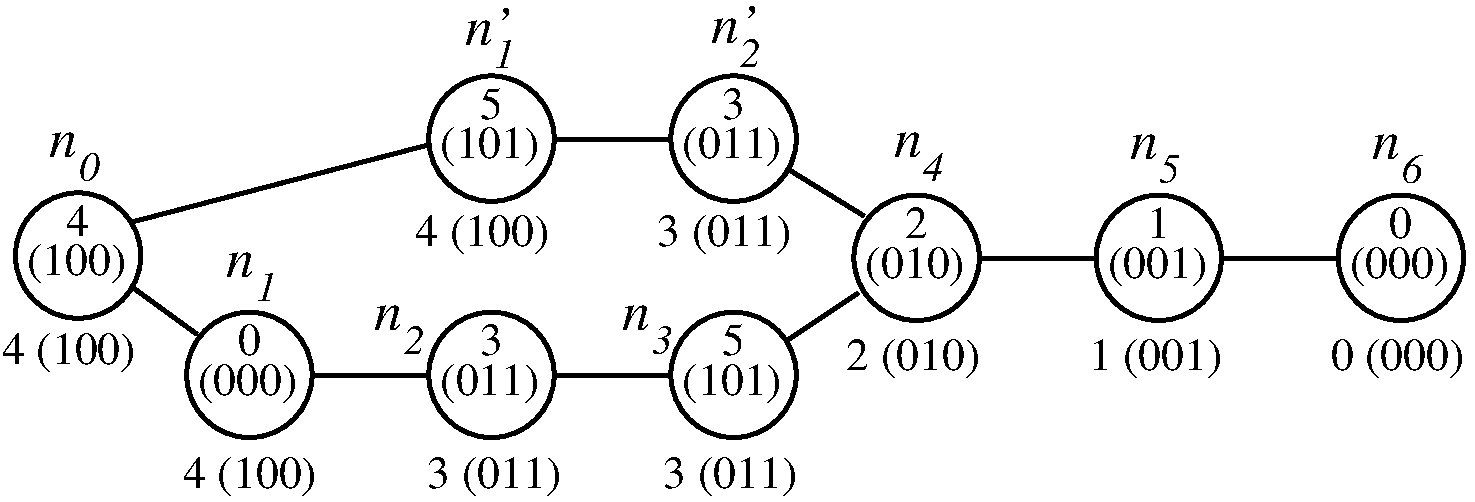
\includegraphics[width=240px]{figures/corruption_example5.pdf}
%\caption{An example of a unit-cost graph with a corrupted heuristic that was consistent before corruption.}
\caption{An example of a corrupted heuristic.}
\label{fig:corruption_example}
\end{center}
\end{figure}
%[Roni: the font is small, enlarging will be good]] An example of heuristic corruption in an undirected, unit-cost graph where $n_0=n_{\mathrm{init}}$ and $n_6 \in V_{\mathrm{goals}}$. The corrupted heuristic values, including the 3-bit binary representation in parentheses, are shown inside each vertex. The values of the consistent heuristic before the corruption are shown below the vertices.[[Roni: for space, we can just have a small caption here: Example of a corrupted inconsistent heuristic]]}

%In this section, we introduce several methods for detecting that a consistent heuristic has been corrupted.

\subsection{Error Detection}

%The basic error detection method we will use 
Our error detection method 
is based on identifying edges which break the consistency property.
If we know the heuristic was initially consistent before corruption occurred, then the existence of an edge $(n, n')$ on which the heuristic is inconsistent is a clear indication that the heuristic value of either $n$ or $n'$ must have been corrupted.
By simply watching for inconsistent edges, we have a simple and sufficient way to detect errors.
Unfortunately, this approach will not necessarily identify all errors.
For example, consider the edge $(n_0, n_1')$ in Figure \ref{fig:corruption_example}.
The heuristic value of $n_1'$ has been corrupted from a value of $4$ to the inadmissible value of $5$.
As the corrupted heuristic remains consistent on this edge, this approach will not identify this error.
Below, we will show that this error detection scheme is still enough for guaranteeing bounded suboptimal solutions. 

% TODO: PUT THIS SOMEWHERE
%Note that in undirected graphs, we can additionally identify a corruption if $H(p) > H(n) - \kappa(p, n)$ where $n$ is the child of $p$.
%This additional check would also allow us to identify that there is a corruption of one of $H(n_0)$ or $H(n_1)$ in Figure \ref{fig:corruption_example}.




%The basic corruption detection methods we propose is to identify a corruption by detecting that a heuristic of a node $n$ is no longer consistent with the heuristic of its parent $p$. We say that a node $n$ is \textbf{locally consistent} with its neighbor $n'$ if $|H(n)-H(n')|\leq \kappa(n,n')$. Following Definition~\ref{def:consistency}, a heuristic is consistent iff it is locally consistent for every pair of adjacent nodes. 

%As an example of the impact that radiation can have on a heuristic, consider the undirected, unit-cost graph in Figure \ref{fig:corruption_example}.
%The uncorrupted heuristic values for $n_0$ through $n_6$ are shown below the nodes, with the 3-bit binary representation shown in parentheses. The heuristic values found after the corruption are shown inside each node. While the original heuristic is consistent, the corrupted heuristic is not.


%Radiation may cause a consistent heuristic to be inconsistent. For example, consider the undirected, unit-cost graph in Figure \ref{fig:corruption_example}. $n_0$ is the initial state and $n_6$ is the goal state. 
%The uncorrupted heuristic values for $n_0$ through $n_6$ are shown below the nodes, with the 3-bit binary representation shown in parentheses. The heuristic values found after the corruption are shown inside each node. While the original heuristic is consistent, the corrupted heuristic is not. For example, $n_0$ is not locally consistent, since $|H(n_0)-H(n_1)| = 4 > 1 = \kappa(n_0, n_1)$, where $H$ is the corrupted heuristic. Since the original heuristic was known to be consistent, we can infer that at least one of the PDB entries used to compute $H(n_3)$ and $H(n_4)$ is corrupted. Lemma~\ref{lem:sufficient-condition} states this observation in a general manner.


%\begin{lemma}[Sufficient condition for corruption detection] 
%If two neighboring nodes $n$ and $n'$ are not locally consistent then at least one of these nodes has a corrupted heuristic value. 
%\label{lem:sufficient-condition}
%\end{lemma}
%Unfortunately, Lemma~\ref{lem:sufficient-condition} only provide sufficient conditions for a corruption to be detected, as corrupted heuristic values that do not violate local consistency will not be detected. 

%
%\subsection{Inadmissible Error Detection}
%
%While errors can degrade the quality of a heuristic when it decreases the heuristic value of a node, it can be even more harmful when it introduces inadmissibility.
%This is because inadmissibility may decrease the quality of solutions we find. % and may make nodes along the solution paths look much less promising than they actually are.
%Thus we focus on detecting when the corrupted heuristic has become inadmissible.
%%For this purpose, 
%Consider the following lemma:
%%A corrupted entry in a PDB can result in either decreasing or increasing the heuristic value. If the heuristic value decreased from its original admissible value, then the search will be slower but the solution quality would still be optimal. If, however, the heuristic value increased, it may have become in admissible. Thus, we focus on detecting cases where the corrupted PDB has caused the heuristic to be inadmissible. 
%
%
%\begin{lemma}%[Inadmissible corruption]
%\label{lemma:inad_corruption}
%If a heuristic $h$ is consistent on every $(n, c)$ where $c \in children(n)$ for some node $n$ and $h(n)>h^*(n)$, 
%%If $H(n)>h^*(n)$ and $n$ is locally consistent with all its children 
%then there exists a node $c \in children(n)$ such that $h(c) > h^*(c)$. 
%\label{lem:inadmissible-corruption}
%\end{lemma}
%\begin{proof}
%Let $c$ be a node on an optimal path from $n$ to a goal.
%Thus, $h^*(n)=h^*(c)+\kappa (n,c)$. Since $h$ is consistent on the edge $(n, c)$, then $h(n)\leq h(c)+\kappa(n,c)$. Together with the inadmissibility of $h(n)$ this means the following:
%\[ h^*(c)+\kappa(n,c)= h^*(n) < h(n) \leq h(c)+\kappa(n,c) \]
%Therefore $h^*(c)<h(c)$ as required.
%\end{proof}
%
%Now we %will extend the definition of a heuristic being consistent on an edge to 
%define the concept of 
%a heuristic being consistent along a path:
%
%\begin{definition}[Path Consistency]
%A heuristic $h$ is said to be consistent along a path of nodes $\pi=[n_0,..,n_k]$ iff $h$ is consistent on every edge along $\pi$. 
%\end{definition}
%Notice that this definition is weaker than consistency and simply requires that for every pair of parent and child nodes on $\pi$, the heuristic never differs by more than the cost of the edge between them.
%For example, note that the corrupted heuristic in Figure \ref{fig:corruption_example} is consistent along $[n_0, n_1']$ as there are no restrictions on how the heuristic value drops from parent to child, but it is not consistent along $[n_0, n_1', n_2']$.
%
%We can now use Lemma \ref{lemma:inad_corruption} to show the following theorem, though the proof is ommitted for space:
%%This definition will now be used in the following theorem which can be proved using Lemma \ref{lemma:inad_corruption}.
%%However, the proof is omitted for space.
%
%\begin{theorem}%[Inadmissible corruption detection] 
%Let $h$ be a state-based heuristic function and let $U$ be an upper bound on the number of states with inadmissible heuristic values.
%If $h$ is consistent along every path $\pi$ that starts at a node $n$ and contains at most $U$ edges, %steps from $n$, 
%then $h(n)$ is admissible.
%%Let $\delta$ be an upper bound on the number of PDB entries that were corrupted. 
%%For any state $n$, if $H$ is locally consistent for every adjacent nodes that are less than $\delta+1$ steps from $n$, then $H(n)$ is admissible.
%\label{the:inadmissible-detection}
%\end{theorem}
%
%Theorem~\ref{the:inadmissible-detection} shows that we can identify all heuristic errors that cause heuristic inadmissibility by performing a $U$ step lookahead from every node. 
%%Thus, if no corruption was detected throughout the search, the found solution is guaranteed to be optimal. 
%However, practically applying this detection method is problematic. First, for a given branching factor $b$, it requires a lookahead with an overhead of $b^{U+1}$ per node, which is not feasible for any non-trivial $U$. Second, as mentioned before, $U$ is hard to compute or approximate for state space search problems. 
%%and while some probabilistic notion of how likely is each $U$ value can be computed by some model of radiation, it is not clear how to compute a definitive upper bound on the number of corrupted entries.
%






%\section{Error Correction}
%For the reasons given above, the sufficient error detection method that only considers the inconsistency of $h$ on edges is more practically applicable than the complete condition given in Theorem~\ref{the:inadmissible-detection}. 
%In this section, we will identify a family of simple error correction methods that can be applied whenever an error is detected and which have a bound on the suboptimality of the found solution.
%We begin by laying the theoretical foundation for this bound.
%However, since some corrupted heuristic values may not be detected with these conditions, the quality of the resulting solution is unbounded. Below we show a family of simple \textbf{corruption correction methods} that can be applied during the search and result in having a bound on the suboptimality of the found solution. Next, we lay the theoretical foundation for these corruption correction methods. 



%\subsection{Bounding Solution Quality}
%Once heuristic corruption has been detected, we need a policy for handling it. In this section, we identify two conditions for any such policy that will be sufficient for guaranteeing that any solution found will cost at most $3\cdot C^*$.


\subsection{Correction with Suboptimality Guarantees}

Let us now identify sufficient conditions for an error correction method that will allow us to guarantee bounded suboptimality.
Informally, the basis for the proposed error correction methods is that by making the corrupted heuristic ``more consistent'' then the corrupted heuristics will not become too incorrect.
In this section, we identify conditions for such correction methods that will ensure that the solutions found are not too suboptimal.
This is done by the following theorems which state that if the heuristic is always consistent along the path to a node when it is evaluated, then any solution found by IDA* will cost no more than $3 \cdot C^*$. 

%\begin{definition}[Path Consistency]
%A node $n$ representing a path $\pi=[n_0,..,n_k]$ in the state space is said said to be path-consistent w.r.t $H$ iff every pair of nodes $n_i,n_i+1\in \pi$ are locally consistent w.r.t $H$. 
%\end{definition}
%The following theorem states that if every expanded node is path consistent then any solution found by IDA* (using $g(n)+H(n)$ as an evaluation function) will cost no more than $3 \cdot C^*$. 

\begin{theorem} (Valenzano et al.~\shortcite{Valenzano:alternative_bounding})
IDA* using the $g+h$ evaluation function will find a solution with a cost of at most $M\cdot C^*$ provided that $g(n) + h(n) \leq M \cdot (g(n)+h^*(n))$ is true for any node $n$ on an optimal path to a goal node. %representing a path of states $[s_0, \cdots, s_k]$ where $s_k$ is along an optimal path.
\label{theorem:rickmas}
\end{theorem}

\begin{theorem}
Any solution found by IDA* will have a cost of at most $3 \cdot C^*$ if (1) $h(n_{\mathrm{init}}) \leq h^*(n_{\mathrm{init}})$ and (2) $h$ is consistent along the path to a node $n$ when $n$ is evaluated.
\label{the:h_increase_policy}
\end{theorem}
\begin{proof}
%In Theorem 2.5 of Valenzano et al.~\shortcite{Valenzano:alternative_bounding}, it was shown that any solution found by an IDA* that uses the $g+H$ evaluation function will have a cost of at most $3\cdot C^*$ provided the following is true: $g(n) + H(n) \leq 3(g(n)+h^*(n))$ for any $n$ that represents a path of states $[s_0, ..., s_k]$ where $s_k$ is along an optimal path.
%As such, we now show that this is true if the two conditions given in the theorem statement hold.
%
%To do so, 
Let $n$ be a node on an optimal path %representing a path whose last state is along some optimal path, 
and let $\pi$ be the path of nodes to $n$.
Notice that by our assumption that $h$ is consistent along $\pi$, the heuristic values can only increase by the edge cost between each pair of consecutive nodes on $\pi$.
As the total of these heuristic increases can be at most the sum of the edge costs (i.e., $g(n)$), this means that $h(n)$ can be at most $h(n_{\mathrm{init}}) + g(n)$.

Now since $h(n) \leq h(n_{\mathrm{init}}) + g(n)$ it follows that $g(n) + h(n) \leq 2 \cdot g(n) + h(n_{\mathrm{init}})$. This also means that $g(n) + h(n) \leq 2 \cdot g(n) + h^*(n_{\mathrm{init}})$ by the assumption that $h$ is admissible on $n_{\mathrm{init}}$.
Since $n$ and $n_{\mathrm{init}}$ are on an optimal path, we then have that $g(n) + h(n) \leq 2 \cdot g(n) + g^*(n) + h^*(n)$.
Since $g(n) \geq g^*(n)$, this simplifies to $g(n) + h(n) \leq 3 \cdot g(n) + h^*(n)$ which is the result that we want. This inequality, along with Theorem 
~\ref{theorem:rickmas} 
%2.5 of Valenzano \textit{et al.}~\shortcite{Valenzano:alternative_bounding} therefore 
proves the desired result.
\end{proof}

% OLD PROOF STUFF
%This allows for the following:
%
%$H(n)$ can be at most $g(n)$ larger than $H(n_{\mathrm{init}})$ since the heuristic could only increase by the edge cost along every edge on the path to $n$. and let $\pi = [n_0, ..., n_k]$ be the path to $n$ where $n_0 = n_{\mathrm{init}}$ and $n_k = n$.
%
%Since $H$ is consistent along $\pi$, for every $0 \leq i < k$, $H(n_{i+1})$ can be at most $\kappa(n_i, n_{i+1})$ larger than $H(n_i)$.
%As such, the most that $H(n)=H(n_k)$ can be larger than $H(n_{\mathrm{init}})$
%Since every expanded node $n$ is path-consistent w.r.t $H$, then $H(n)$ cannot be larger from $H(n_{\mathrm{init}})$ by more than $g(n)$. 
%Therefore:
%
%\begin{align}
%g(n) + H(n) &\leq 2\cdot g(n) + H(n_{\mathrm{init}})\label{line:g_as_max1}\\ 
%& \leq 2 \cdot g(n) + h^*(n_{\mathrm{init}})\label{line:g_as_max2}\\
%& \leq 2 \cdot g(n) + g^*(n) + h^*(n)\label{line:g_as_max3}\\
%& \leq 3 \cdot g(n) + h^*(n) \label{line:g_as_max4}\\
%& \leq 3(g(n) + h^*(n))\label{line:g_as_max5}
%\end{align}
%Line \ref{line:g_as_max2} holds because by the heuristic of the initial state is assumed to be admissible. Line \ref{line:g_as_max3} follows from 
%$h^*(n_{\mathrm{init}})$ being the optimal solution, and thus the optimal path passing via $n$ (=$g^*(n) + h^*(n)$) cannot have a lower cost.
%Since the cost of the optimal path to $n$ must be no more costly than the path found, $g^*(n)\leq g(n)$, which implies line \ref{line:g_as_max4}.
%The last line then follows immediately.


%In Theorem 2.5 of Valenzano et al.~\shortcite{Valenzano:alternative_bounding} it was shown that any solution found by an IDA* that uses the $g+H$ evaluation function will have a cost of at most $3\cdot C^*$ if $g(n) + H(n) \leq 3(g(n)+h^*(n))$ for any $n$ along an optimal path.
%Therefore, the statement holds by line \ref{line:g_as_max5} and Theorem 2.5 of Valenzano et al.~\shortcite{Valenzano:alternative_bounding} .
%return a solution that costs iterative deepening search algorithm that uses an evaluation function $F(n)\leq B(g(n)+h^*(n))$ is guaranteed to return a solution that is at most $B(C^*)$ for any bounding function. The $g(n)+H(n)$ evaluation function is a special case where $F(n)=g(n)+H(n)$ and the bounding function $B$ is $B(x)=3\cdot x$


The practical implications of Theorem~\ref{the:h_increase_policy} are that it identifies two conditions for our correction methods for guaranteeing any solution found with cost at most $3 \cdot C^*$. The first requires that $h$ is admissible for $n_{\mathrm{init}}$. To ensure this, recall that the PDB is stored in slow-access reliable memory before search.
We can therefore make a single access to this memory to get an admissible estimate for $n_{\mathrm{init}}$ and store it in reliable DRAM to satisfy this condition. 
To satisfy the condition that $h$ is consistent along every path, we simply need to design the correction methods appropriately. This is done in the next section. 
%We emphasize that while there are 
The correction methods we present next can be used with optimal algorithms such as IDA*, as well as with 
linear-space bounded suboptimal search algorithms such as Weighted IDA*, and Weighted RBFS~\cite{Korf1992}. % and RBFS$_{ktrht}$~\cite{hatem2015recursive}. % these algorithms are not resilient to errors, and can return solutions that are arbitrarily suboptimal when guided by PDBs stored in unreliable memory. 







%Notice that the resulting bound holds regardless of the amount of heuristic corruption or whether the domain is undirected or not. 


\subsection{Correction Methods}

%In this section, we will introduce heuristic correction methods that will be applied whenever our approximate corruption detection algorithm %the corruption detection technique described in Section \ref{sec:corruption_detection} 
%suggests a corruption has occurred. 
%Like that technique, these correction methods are designed with the fact that the corrupted PDB heuristic was originally consistent before it was corrupted.


%An important property of these conditions is that they may only be violated if the approximate corruption detection method based on Lemma~\ref{lem:sufficient-condition}. Thus, we can obtain the desired factor 3 suboptimality bound by applying the correction techniques described below only when a corruption was identified using Lemma~\ref{lem:sufficient-condition}, which, as discussed above, is easy to implement. 




%In this section, we introduce several error correction methods. Roni: repetition of the last sentence

%As we continue to use the corrupted PDB in Figure \ref{fig:corruption_example} as a running example, we will use $PDB(n)$ to denote the possibly corrupted state-based heuristic value returned by the PDB, and $h(n)$ to denote the (possibly corrected) path-based heuristic value used for evaluating nodes during search. As such, $PDB(n)$ refers to the heuristic value shown inside each node in Figure \ref{fig:corruption_example}. However, we stress that similar approaches could be used for other memory-based heuristics (in which case $PDB(n)$ would refer to the heuristic value returned by the corrupted memory-based heuristic). Roni: very wordy 

Let $PDB(n)$ and $h(n)$ refers to the possibly corrupted heuristic value of $n$ and the heuristic value of $n$ after applying one of the detailed below correction methods, respectively. In the example in Figure~\ref{fig:corruption_example}, $PDB(n)$ is the number inside each node.\footnote{We use the $PDB(n)$ notation for clarity, but our approach applies to any memory-based heuristic.}  
%\roni{Where is $h(n)$ stored?}


% 
The correction methods below work as follows: when a node $n$ is generated expanding node $p$, then the possibly corrupted heuristic of $n$  ($PDB(n)$) is compared with the corrected heuristic of $p$ ($h(p)$). If $|h(p) - PDB(n)| > \kappa(p, n)$, we will use our correction methods to select a value for $h(n)$ that is in the range $[h(p)-\kappa(p,n),h(p)+\kappa(p,n)]$.
We will denote this range by $P_{p,n}$.
By setting $h(n)$ so it is $P_{p,n}$ will ensure that if $h$ is consistent along the path to $p$ (which it must be by an inductive argument), then $h$ will also be consistent along the path to $n$. 
Thus, any solution found when using the correction methods described below will cost at most $3 \cdot C^*$  by Theorem \ref{the:h_increase_policy}.


%\roni{The above paragraph is over-confusing. My suggestion is to state this as a theorem, something like this: if when $n$ is generated by $p$ its heuristic is set to $h(n)$ such that $h(n)\in P_{p,n}$ then the path $n$ is edge consistent. Then say that next we propose several methods that implement this rule, differing in which value to choose from $P_{p,n}$.} 


% Last version
%All correction methods described below are applied when a node is generated, and satisfy the conditions of Theorem \ref{the:h_increase_policy} and thus result in a bounded solution quality. 
%
%To avoid confusion between the corrupted heuristic and the heuristic value after correction we denote by $PDB(n)$  as the possibly corrupted state-based heuristic value returned by the PDB, and denote by $H(n)$ the (possibly corrected) path-based heuristic value used during the search.
%When referring to Figure \ref{fig:corruption_example}, this means that $PDB(n)$ returns the heuristic value shown inside each node.




%Notice that this means $H(n)=PDB(n)$ when no corruption is detected. Hereonafter, we say that a corruption is detected at a node $n$ if $H$ is not neighborhood consistent for $n$ (following Lemma~\ref{lem:sufficient-condition}).


%If $H(n)\leq PDB(n')+\kappa(n,n')$ set $H(n')=PDB(n') Else, set $H(n')$ to be any value such that $PDB(n')\geq H(n)-\kappa(n,n')$

%Deriving practical correction methods from the conditions of Theorem \ref{the:h_increase_policy} raises two design choices: (1) when to apply the correction method, i.e., how to detect a possible corruption, and (2) how to corrected a possibly corrupted heuristic value.


\subsubsection{Parent-Based Corrections}
The first family of error correction methods we consider, referred to as ``parent-based'', set $h(n)$ as a function of $h(p)$ and $PDB(n)$. 
%only consult $h(p)$ when selecting a value for $h(n)$ from the range $P_{p,n}$, where $n$ is the node generated by the expansion of $p$ and an error is detected on edge $(p, n)$. 
The first two such methods we propose are the \textbf{pessimistic} method, which sets $h(n)$ as $h(p) + \kappa(p, n)$ when an error is detected, and the \textbf{optimistic} method, which sets $h(n)$ as $h(p) - \kappa(p, n)$. For example, in Figure~\ref{fig:corruption_example} if $n_0$ is the parent of $n_1$, the pessimistic method would set $h(n_1)$ to 5, while the optimistic method would set $h(n_1)$ to 3.

%Let $n$ be the node being generated and let $p$ be its parent. 
%The first type of corruption correction methods is based on two values: the (possibly corrected) heuristic of $p$ ($H(p)$) and the PDB-based heuristic of $n$ ($PDB(n)$). Correction methods of this type are called \textbf{parent-based}. 
%If $|H(p)- PDB(n)|\leq \kappa(p,n)$, parent-based methods set $H(n)$ as $PDB(n)$.%\footnote{This is the undirected version of corruption detection by checking if two adjacent nodes are consistent.} 
%Otherwise, parent-based corrections set $H(n)$ such that $|H(p)- H(n)|\leq \kappa(p,n)$ holds. Let $P_{p,n}$ be this range of values (i.e.,  $P_{p,n}=[H(p)-\kappa(p,n),H(p)+\kappa(p,n)]$).
%
%
%The first two parent-based correction methods we propose are the \textbf{pessimistic} method, which sets $H(n)$ as $H(p) + \kappa(p, n)$ when corruption is detected, and the \textbf{optimistic} method, which sets $H(n)$ as $H(p) - \kappa(p, n)$. For example, in Figure~\ref{fig:corruption_example} if $n_0$ is the parent of $n_1$, the pessimistic method would set $H(n_1)$ to 5, while the optimistic method would set $H(n_1)$ to 3.


% Rick: Can use Figure 1 for examples. H(n_1) will be set as 5 using pessimistic, and then H(n_2) is set as 6. H(n_1) is set as 3 for optimistic, and then H(n_3) will be set 2.

%Use the fact that we are looking at 
%Pessimistic is also increase heuristic from parent to child by cost of edge. Optimistic is the one that always decreases.

The third parent-based correction method we propose attempts to use the value of $h(p)$ to choose the value from $P_{p,n}$ that is most likely to have been the original uncorrupted PDB value. If we assume that corruption is random, then the most likely corruption to $PDB(n)$ is that in which the least bits were flipped. Thus, we set $h(n)$ in this error correction method to the value in $P_{p,n}$ that has the minimal Hamming distance (distance in bit flips) from $PDB(n)$. 
%To do so, we compute the Hamming distance between each value in $P_{p,n}$ and $PDB(n)$. That is, we count the number of bits one would have to flip to transform each value in $P_{p,n}$ into $PDB(n)$. %Since every radiation-caused corruption flips one bit, 
%This approach estimates the number of times $n$'s PDB entry was corrupted. Then we set $h(n)$ to the value in $P_{p,n}$ with the lowest count. 
This approach is inspired by the popular ``minimal cardinality'' method often used in automated diagnosis, which states that when all faults are equally likely, the most likely diagnosis is the one which assumes the least amount of failures~\cite{de1987diagnosing}.
Formally, we set $h(n)$ as follows:
\begin{equation}
h(n) = \underset{v \in P_{p,n}}{\argmin} \, Hamming(v, PDB(n)) \,,
\end{equation}
\noindent
where $Hamming(v, PDB(n))$ is the Hamming distance between the binary representations of $v$ and $PDB(n)$. Ties are broken in favor of the higher value. 
%In the case of ties, $H(n)$ is set as the highest of the tied values. 
We call this method \textbf{Parent Minimum Cardinality Diagnosis Correction (PMCD)}.

As an example of PMCD, consider node $n_1$ in Figure \ref{fig:corruption_example}. When the search arrives at this node from $n_0$ it will detect an error due to the inconsistency of the heuristic on edge $(n_0, n_1)$.
Since $h(n_0)=4$, consistency requires that $h(n_1)$ be set as either 3 (011), 4 (100), or 5 (101). The Hamming distance of each of these from the corrupted $PDB(n_1)$ value of 0 (000) are 2, 1, and 2, respectively.
Therefore, CMCD correction would set $h(n_1)$ correctly as 4.

\subsubsection{Children-Based Corrections}
%\subsubsection{Children Minimum Cardinality Diagnosis Correction}

An alternative type of error correction considers not only $h(p)$ and $PDB(n)$, but also $PDB(c)$ for all $c \in children(n)$. We call this type of correction method a \textbf{children-based} correction method. 
%
As in the parent-based correction methods, children-based correction only considers a value other than $PDB(n)$ for $h(n)$ if $PDB(n)$ is not in $P_{p,n}$. When that occurs, we use the following voting mechanism to take into consideration the values of $PDB(c)$ when setting $h(n)$. 
Let $C_{n,c}=[PDB(c)-\kappa(n,c),PDB(c)+\kappa(n,c)]$, i.e., the value expected for $n$ in order $h$ to be consistent along the edge from $n$ to $c$. In addition, let $UC_{h(n)}$ be the union of all possible heuristic values $h(n)$ could assume according to $n$'s children, i.e., $UC_n = \bigcup_{c \in children(n)} C_{n,c}$.

For every value $v\in UC_n$, let $CC(v)$ be the number of children of $n$ such that if $h(n)=v$ then $h$ would be consistent on those edges, where the children of $n$ that are mapped to the same PDB entry are counted only once. We then set $h(n)$ to be the value $v$ that maximizes $CC(v)$, where ties are broken in favor of the value that is closest to $PDB(n)$ in terms of Hamming distance.
If the value that maximizes $CC(v)$ is outside the range of $C_{p,c}$, $h(n)$ is set to $h(p) + k(p, n)$ in order to preserve the $3 \cdot C^*$ suboptimality bound.
We call this children-based correction method \textbf{Child Minimum Cardinality Diagnosis Correction (CMCD)}. 

The intuition behind CMCD is similar to PMCD: set $h(n)$ to be the value that assumes the least amount of failures in PDB entries, though in this case we consider the PDB entries of its children. 
As an example, consider the path $[n_0, n_1, n_2, n_3]$ in Figure~\ref{fig:corruption_example}.
As the reader can verify, CMCD will correctly set $h(n_1)$ as $4$, and so the next error discovered will be on edge $(n_2, n_3)$. 
Since $h(n_2)$ is $3$  and $PDB(n_4)$ is $2$, $UC_{n_3} = \{1, 2, 3, 4\}$ and $CC(1)=1$, $CC(2)=2$, $CC(3)=2$, and $CC(4)=1$.
The tie between $v=2$ and $v=3$ is broken by computing the Hamming distance between 2 (010), and 5 (101) and between 3 (011) and 5 (101). Since 3 is closer to 5 in terms of Hamming distance, CMCD correctly sets $h(n_3)$ to $3$.
This is unlike PMCD which will incorrectly set $h(n_3)$ to $4$.

%\begin{example}
%Let us consider the graph in Figure~\ref{fig:corruption_example}. We would like to correct the corrupted $H$-value of $n_3$ ($H(n_3) = 7$). Assume that the heuristic of it neighbors ($n_2$, $n_4$, $n_4'$) is not corrupted. If we have unit-edge costs, then $UC_{n_3} = \{1, 2, 3, 4\}$, and $CC(1)=1$, $CC(2)=2$, $CC(3)=2$, and $CC(4)=1$.
%The tie between $v=2$ and $v=3$ is broken by computing the Hamming distance between 2 (0010) and 7 (0111) and between 3 (0011) and 7 (0111). Since 3 is closer to 7 in terms of Hamming distance, CMCD correctly sets $H(n_3)$ to $3$. 
%\end{example}
Note that the children-based methods need a small one-step lookahead to obtain $PDB(c)$ for all children of $n$, and thus incurs more overhead than the parent-based methods. 



% Rick: Can use Figure 1 for examples. H(n_5) doesn't need Hamming distance. Hamming distance breaks tie in n_3

%\subsubsection{Child Hamming Distance Correction (Voting?) (Min Diagnosis?)}

%\subsubsection{PDB Updating}
%[Levi: Are we doing updating after all?]
%[Rick: I wasn't sure, so I just made a header for it. We can get rid of it to simplify things. Levi: OK, let's write without it and then see how it looks]

%\section{Methodology}
%
%In this paper we assume there is a limited amount of protected memory available. 



\section{Empirical Evaluation}

%We begin with a description of our experimental methodology and then discuss the results.
%Due to space limitations, we omit from our table the results of the optimistic approach. We discuss the omitted results in the text, nevertheless. In this section, when we write IDA*, we refer to the search algorithm which does not use any correction method.
%We refer to IDA* using correction algorithm ``X'' simply as ``X''. When we write IDA* we refer to the search algorithm without any correction technique.
\begin{table}[t]
\centering
\footnotesize
\setlength{\tabcolsep}{4.0 pt}
\begin{tabular}{| c | r  r | r  r | r  r | r  r |}
\hline
\multicolumn{9}{|c|}{\textbf{15-Pancake puzzle}} \\
\hline
FPNE     & \multicolumn{2}{|c|}{IDA*}    & \multicolumn{2}{|c|}{Pessimistic}     & \multicolumn{2}{|c|}{PMCD}    & \multicolumn{2}{|c|}{CMCD}    \\
\hline
        & \multicolumn{1}{c}{Cov.} & \multicolumn{1}{c|}{Sub.}        & \multicolumn{1}{c}{Cov.} & \multicolumn{1}{c|}{Sub.}        & \multicolumn{1}{c}{Cov.} & \multicolumn{1}{c|}{Sub.}        & \multicolumn{1}{c}{Cov.} & \multicolumn{1}{c|}{Sub.}        \\
\hline
%$10^{0}$         & 0.00  & -     & 0.03         & 1.00         & 0.00        & -         & 0.03         & 1.08        \\
$10^{-1}$        & 0.13  & 1.10  & 1.70         & 1.06         & 1.37         & 1.00         & 2.40         & 1.01        \\
$10^{-2}$        & 2.93  & 1.03  & 5.57         & 1.04         & 4.87         & 1.00         & 4.00         & 1.00        \\
$10^{-3}$        & 6.43  & 1.01  & 12.97        & 1.02         & 7.77         & 1.00         & 5.00  & 1.00 \\
$10^{-4}$        & 9.13  & 1.00  & 10.43       & 1.00         & 9.83         & 1.00        & 7.50  & 1.00 \\
$10^{-5}$        & 9.83  & 1.00  & 9.80  & 1.00  & 10.00        & 1.00         & 9.83         & 1.00        \\
$10^{-6}$	 & 9.93	 & 1.00	 & 10.00	 & 1.00	 & 10.00	 & 1.00	 & 10.00	 & 1.00	\\
$10^{-7}$	 & 10.00	 & 1.00	 & 10.00	 & 1.00	 & 10.00	 & 1.00	 & 10.00	 & 1.00	\\
0        & 10.00         & 1.00          & 10.00        & 1.00         & 10.00        & 1.00         & 10.00        & 1.00        \\
\hline
\hline
\multicolumn{9}{|c|}{\textbf{(17,4)-Topspin puzzle}} \\
\hline
FPNE     & \multicolumn{2}{|c|}{IDA*}    & \multicolumn{2}{|c|}{Pessimistic}     & \multicolumn{2}{|c|}{PMCD}    & \multicolumn{2}{|c|}{CMCD}    \\
\hline
        & \multicolumn{1}{c}{Cov.} & \multicolumn{1}{c|}{Sub.}  & \multicolumn{1}{c}{Cov.} & \multicolumn{1}{c|}{Sub.}  & \multicolumn{1}{c}{Cov.} & \multicolumn{1}{c|}{Sub.}  & \multicolumn{1}{c}{Cov.} & \multicolumn{1}{c|}{Sub.}  \\
\hline
%$10^{0}$         & 3.57  & 1.00  & 4.89         & 1.00         & 1.97  & 1.00  & 2.73  & 1.00 \\
$10^{-1}$        & 5.68  & 1.00  & 9.45         & 1.00         & 3.83  & 1.00  & 3.03  & 1.00 \\
$10^{-2}$        & 6.33  & 1.00  & 9.00         & 1.00         & 5.03  & 1.00  & 4.83  & 1.00 \\
$10^{-3}$        & 6.03  & 1.00  & 6.00  & 1.00  & 5.93  & 1.00  & 5.23  & 1.00 \\
$10^{-4}$        & 6.00  & 1.00  & 6.00         & 1.00         & 6.00         & 1.00         & 6.00         & 1.00        \\
$10^{-5}$        & 6.00  & 1.00  & 6.00         & 1.00         & 6.00         & 1.00         & 6.00         & 1.00        \\
$10^{-6}$	 & 6.00	 & 1.00	 & 6.00	 & 1.00	 & 6.00	 & 1.00	 & 6.00	 & 1.00	\\
$10^{-7}$	 & 6.00	 & 1.00	 & 6.00	 & 1.00	 & 6.00	 & 1.00	 & 6.00	 & 1.00	\\
0        & 6.00  & 1.00          & 6.00         & 1.00         & 6.00         & 1.00         & 6.00         & 1.00        \\
\hline
\hline
\multicolumn{9}{|c|}{\textbf{(4x4) Sliding-Tile puzzle}} \\
\hline
FPNE     & \multicolumn{2}{|c|}{IDA*}    & \multicolumn{2}{|c|}{Pessimistic}     & \multicolumn{2}{|c|}{PMCD}    & \multicolumn{2}{|c|}{CMCD}    \\
\hline
        & \multicolumn{1}{c}{Cov.} & \multicolumn{1}{c|}{Sub.}  & \multicolumn{1}{c}{Cov.} & \multicolumn{1}{c|}{Sub.}  & \multicolumn{1}{c}{Cov.} & \multicolumn{1}{c|}{Sub.}  & \multicolumn{1}{c}{Cov.} & \multicolumn{1}{c|}{Sub.}  \\
\hline
%$10^{0}$         & 4.90  & 1.01  & 5.17         & 1.01         & 8.80         & 1.01         & 7.33         & 1.00        \\
$10^{-1}$        & 9.33  & 1.02  & 8.87  & 1.01  & 12.93        & 1.00         & 12.37        & 1.00        \\
$10^{-2}$        & 15.07         & 1.95  & 14.13         & 1.01  & 19.13        & 1.00         & 18.03        & 1.00        \\
$10^{-3}$        & 22.00         & 1.02  & 20.97         & 1.01  & 21.50         & 1.00  & 20.63         & 1.00 \\
$10^{-4}$        & 22.10         & 1.00  & 21.80         & 1.00  & 21.93         & 1.00  & 21.80         & 1.00 \\
$10^{-5}$        & 22.10         & 1.00  & 22.13        & 1.00         & 22.00         & 1.00  & 22.03         & 1.00 \\
$10^{-6}$	 & 22.67	 & 1.00	 & 22.80	 & 1.00	 & 22.50	 & 1.00	 & 22.67	 & 1.00	\\
$10^{-7}$	 & 23.00	 & 1.00	 & 22.90	 & 1.00	 & 22.90	 & 1.00	 & 22.97	 & 1.00	\\
0        & 23.00         & 1.00          & 23.00        & 1.00         & 23.00        & 1.00         & 23.00        & 1.00        \\
\hline
%\hline
%\multicolumn{9}{|c|}{\textbf{(5x5) Sliding-Tile puzzle}} \\
%\hline
%FPNE     & \multicolumn{2}{|c|}{IDA*}    & \multicolumn{2}{|c|}{Pessimistic}     & \multicolumn{2}{|c|}{PMCD}    & \multicolumn{2}{|c|}{CMCD}    \\
%\hline
%        & \multicolumn{1}{c}{Cov.} & \multicolumn{1}{c|}{Sub.}  & \multicolumn{1}{c}{Cov.} & \multicolumn{1}{c|}{Sub.}  & \multicolumn{1}{c}{Cov.} & \multicolumn{1}{c|}{Sub.}  & \multicolumn{1}{c}{Cov.} & \multicolumn{1}{c|}{Sub.}  \\
%\hline
%%$10^{0}$	 & 0.07	 & 1.00	 & 0.33	 & 1.00	 & 0.00	 & - 	 & 0.60	 & 1.01	\\
%$10^{-1}$	 & 2.60	 & 1.00	 & 2.93	 & 1.00	 & 3.13	 & 1.00	 & 3.07	 & 1.01	\\
%$10^{-2}$	 & 4.33	 & 1.00	 & 4.80	 & 1.00	 & 3.93	 & 1.00	 & 4.13	 & 1.00	\\
%$10^{-3}$	 & 4.93	 & 1.00	 & 4.40	 & 1.00	 & 4.47	 & 1.00	 & 5.07	 & 1.00	\\
%$10^{-4}$	 & 5.53	 & 1.00	 & 5.93	 & 1.00	 & 5.47	 & 1.00	 & 5.33	 & 1.00	\\
%$10^{-5}$	 & 5.13	 & 1.00	 & 5.33	 & 1.00	 & 5.47	 & 1.00	 & 5.87	 & 1.00	\\
%$10^{-6}$	 & 7.00	 & 1.00	 & 7.80	 & 1.00	 & 6.73	 & 1.00	 & 6.80	 & 1.00	\\
%$10^{-7}$	 & 7.47	 & 1.00	 & 7.80	 & 1.00	 & 7.87	 & 1.00	 & 8.27	 & 1.00	\\
%0 	 & 8.33	 & 1.00 	 & 7.13	 & 1.00 	 & 7.00	 & 1.00 	 & 6.87	 & 1.00 	\\
%\hline
\end{tabular}
%\caption{The table shows the average number of problems solved and the average suboptimality of the different correction algorithms on the puzzle, pancake, topspin domains. A bold entry means that that correction algorithm was able to solve more or the same number of problems on average than IDA*.}
\caption{Results for different levels of simulated radiation when consistent heuristics are employed.}
\label{tab:results}
\end{table}


\begin{table}[t]
\centering
%\footnotesize
\setlength{\tabcolsep}{4.0 pt}
\begin{tabular}{| c | r  r | r  r | r  r | r  r |}
\hline
\multicolumn{9}{|c|}{\textbf{(5x5) Sliding-Tile puzzle}} \\
\hline
FPNE     & \multicolumn{2}{|c|}{IDA*}    & \multicolumn{2}{|c|}{Pessimistic}     & \multicolumn{2}{|c|}{PMCD}    & \multicolumn{2}{|c|}{CMCD}    \\
\hline
        & \multicolumn{1}{c}{Cov.} & \multicolumn{1}{c|}{Sub.}  & \multicolumn{1}{c}{Cov.} & \multicolumn{1}{c|}{Sub.}  & \multicolumn{1}{c}{Cov.} & \multicolumn{1}{c|}{Sub.}  & \multicolumn{1}{c}{Cov.} & \multicolumn{1}{c|}{Sub.}  \\
\hline
%$10^{0}$	 & 0.07	 & 1.00	 & 0.33	 & 1.00	 & 0.00	 & - 	 & 0.60	 & 1.01	\\
$10^{-1}$	 & 2.60	 & 1.00	 & 2.93	 & 1.00	 & 3.13	 & 1.00	 & 3.07	 & 1.01	\\
$10^{-2}$	 & 4.33	 & 1.00	 & 4.80	 & 1.00	 & 3.93	 & 1.00	 & 4.13	 & 1.00	\\
$10^{-3}$	 & 4.93	 & 1.00	 & 4.40	 & 1.00	 & 4.47	 & 1.00	 & 5.07	 & 1.00	\\
$10^{-4}$	 & 5.53	 & 1.00	 & 5.93	 & 1.00	 & 5.47	 & 1.00	 & 5.33	 & 1.00	\\
$10^{-5}$	 & 5.13	 & 1.00	 & 5.33	 & 1.00	 & 5.47	 & 1.00	 & 5.87	 & 1.00	\\
$10^{-6}$	 & 7.00	 & 1.00	 & 7.80	 & 1.00	 & 6.73	 & 1.00	 & 6.80	 & 1.00	\\
$10^{-7}$	 & 7.47	 & 1.00	 & 7.80	 & 1.00	 & 7.87	 & 1.00	 & 8.27	 & 1.00	\\
0 	 & 8.33	 & 1.00 	 & 7.13	 & 1.00 	 & 7.00	 & 1.00 	 & 6.87	 & 1.00 	\\
\hline
\end{tabular}
\caption{Results for different levels of simulated radiation when an inconsistent heuristic is employed.}
\label{tab:24puzzle}
\end{table}

% \begin{table*}[t]
% \centering
% \begin{tabular}{| c | r  r | r  r | r  r | r  r | r  r |}
% \hline
% \multicolumn{11}{|c|}{\textbf{15-Pancake Puzzle}} \\
% \hline
% FPNE	& \multicolumn{2}{|c|}{Standard IDA*} 	& \multicolumn{2}{|c|}{Pessimistic} 	& \multicolumn{2}{|c|}{Optimistic} 	& \multicolumn{2}{|c|}{PMCD} 	& \multicolumn{2}{|c|}{CMCD} 	\\
% \hline
% 	& \multicolumn{1}{c}{Solved} & \multicolumn{1}{c|}{Sub.} 	& \multicolumn{1}{c}{Solved} & \multicolumn{1}{c|}{Sub.} 	& \multicolumn{1}{c}{Solved} & \multicolumn{1}{c|}{Sub.} 	& \multicolumn{1}{c}{Solved} & \multicolumn{1}{c|}{Sub.} 	& \multicolumn{1}{c}{Solved} & \multicolumn{1}{c|}{Sub.} 	\\
% \hline
% $10^{0}$         & 0.00 $\pm$ 0.00       & -     & \textbf{0.03} $\pm$ \textbf{0.01}     & \textbf{1.00}         & 0.00 $\pm$ 0.00     & -         & 0.00 $\pm$ 0.00     & -         & \textbf{0.03} $\pm$ \textbf{0.01}     & \textbf{1.08}        \\
% $10^{-1}$        & 0.13 $\pm$ 0.01       & 1.10  & \textbf{1.70} $\pm$ \textbf{0.04}     & \textbf{1.06}         & 0.00 $\pm$ 0.00       & -     & \textbf{1.37} $\pm$ \textbf{0.02}     & \textbf{1.00}         & \textbf{2.40} $\pm$ \textbf{0.03}     & \textbf{1.01}        \\
% $10^{-2}$        & 2.93 $\pm$ 0.04       & 1.03  & \textbf{5.57} $\pm$ \textbf{0.05}     & \textbf{1.04}         & 0.00 $\pm$ 0.00       & -     & \textbf{4.87} $\pm$ \textbf{0.01}     & \textbf{1.00}         & \textbf{4.00} $\pm$ \textbf{0.00}     & \textbf{1.00}        \\
% $10^{-3}$        & 6.43 $\pm$ 0.04       & 1.01  & \textbf{12.97} $\pm$ \textbf{0.09}    & \textbf{1.02}         & 0.00 $\pm$ 0.00       & -     & \textbf{7.77} $\pm$ \textbf{0.03}     & \textbf{1.00}         & 5.00 $\pm$ 0.00       & 1.00 \\
% $10^{-4}$        & 9.13 $\pm$ 0.03       & 1.00  & \textbf{10.43} $\pm$ \textbf{0.03}    & \textbf{1.00}         & 0.80 $\pm$ 0.01       & 1.00  & \textbf{9.83} $\pm$ \textbf{0.02}     & \textbf{1.00}         & 7.50 $\pm$ 0.02       & 1.00 \\
% $10^{-5}$        & 9.83 $\pm$ 0.01       & 1.00  & 9.80 $\pm$ 0.02       & 1.00  & 1.50 $\pm$ 0.02       & 1.00  & \textbf{10.00} $\pm$ \textbf{0.00}    & \textbf{1.00}         & \textbf{9.83} $\pm$ \textbf{0.01}     & \textbf{1.00}        \\
% 0        & 10.00 $\pm$ 0.00      & 1.00          & \textbf{10.00} $\pm$ \textbf{0.00}    & \textbf{1.00}         & \textbf{10.00} $\pm$ \textbf{0.00}    & \textbf{1.00}         & \textbf{10.00} $\pm$ \textbf{0.00}    & \textbf{1.00}         & \textbf{10.00} $\pm$ \textbf{0.00}    & \textbf{1.00}        \\
% \hline
% \hline
% \multicolumn{11}{|c|}{\textbf{(17,4)-Topspin Puzzle}} \\
% \hline
% FPNE	& \multicolumn{2}{|c|}{Standard IDA*} 	& \multicolumn{2}{|c|}{Pessimistic} 	& \multicolumn{2}{|c|}{Optimistic} 	& \multicolumn{2}{|c|}{PMCD} 	& \multicolumn{2}{|c|}{CMCD} 	\\
% \hline
% 	& \multicolumn{1}{c}{Solved} & \multicolumn{1}{c|}{Sub.} 	& \multicolumn{1}{c}{Solved} & \multicolumn{1}{c|}{Sub.} 	& \multicolumn{1}{c}{Solved} & \multicolumn{1}{c|}{Sub.} 	& \multicolumn{1}{c}{Solved} & \multicolumn{1}{c|}{Sub.} 	& \multicolumn{1}{c}{Solved} & \multicolumn{1}{c|}{Sub.} 	\\
% \hline
% $10^{0}$         & 3.57 $\pm$ 0.03       & 1.00  & \textbf{4.89} $\pm$ \textbf{0.03}     & \textbf{1.00}         & 0.00 $\pm$ 0.00       & -     & 1.97 $\pm$ 0.01       & 1.00  & 2.73 $\pm$ 0.01       & 1.00 \\
% $10^{-1}$        & 5.68 $\pm$ 0.04       & 1.00  & \textbf{9.48} $\pm$ \textbf{0.06}     & \textbf{1.00}         & 0.00 $\pm$ 0.00       & -     & 3.83 $\pm$ 0.02       & 1.00  & 3.03 $\pm$ 0.01       & 1.00 \\
% $10^{-2}$        & 6.33 $\pm$ 0.03       & 1.00  & \textbf{9.00} $\pm$ \textbf{0.05}     & \textbf{1.00}         & 0.43 $\pm$ 0.02       & 1.00  & 5.03 $\pm$ 0.01       & 1.00  & 4.83 $\pm$ 0.02       & 1.00 \\
% $10^{-3}$        & 6.03 $\pm$ 0.01       & 1.00  & 6.00 $\pm$ 0.00       & 1.00  & 1.80 $\pm$ 0.01       & 1.00  & 5.93 $\pm$ 0.01       & 1.00  & 5.23 $\pm$ 0.01       & 1.00 \\
% $10^{-4}$        & 6.00 $\pm$ 0.00       & 1.00  & \textbf{6.00} $\pm$ \textbf{0.00}     & \textbf{1.00}         & 2.00 $\pm$ 0.00       & 1.00  & \textbf{6.00} $\pm$ \textbf{0.00}     & \textbf{1.00}         & \textbf{6.00} $\pm$ \textbf{0.00}     & \textbf{1.00}        \\
% $10^{-5}$        & 6.00 $\pm$ 0.00       & 1.00  & \textbf{6.00} $\pm$ \textbf{0.00}     & \textbf{1.00}         & 3.80 $\pm$ 0.03       & 1.00  & \textbf{6.00} $\pm$ \textbf{0.00}     & \textbf{1.00}         & \textbf{6.00} $\pm$ \textbf{0.00}     & \textbf{1.00}        \\
% 0        & 6.00 $\pm$ 0.00       & 1.00          & \textbf{6.00} $\pm$ \textbf{0.00}     & \textbf{1.00}         & \textbf{6.00} $\pm$ \textbf{0.00}     & \textbf{1.00}         & \textbf{6.00} $\pm$ \textbf{0.00}     & \textbf{1.00}         & \textbf{6.00} $\pm$ \textbf{0.00}     & \textbf{1.00}        \\
% \hline
% \hline
% \multicolumn{11}{|c|}{\textbf{(4x4) Sliding-Tile Puzzle}} \\
% \hline
% FPNE	& \multicolumn{2}{|c|}{Standard IDA*} 	& \multicolumn{2}{|c|}{Pessimistic} 	& \multicolumn{2}{|c|}{Optimistic} 	& \multicolumn{2}{|c|}{PMCD} 	& \multicolumn{2}{|c|}{CMCD} 	\\
% \hline
% 	& \multicolumn{1}{c}{Solved} & \multicolumn{1}{c|}{Sub.} 	& \multicolumn{1}{c}{Solved} & \multicolumn{1}{c|}{Sub.} 	& \multicolumn{1}{c}{Solved} & \multicolumn{1}{c|}{Sub.} 	& \multicolumn{1}{c}{Solved} & \multicolumn{1}{c|}{Sub.} 	& \multicolumn{1}{c}{Solved} & \multicolumn{1}{c|}{Sub.} 	\\
% \hline
% $10^{0}$         & 4.90 $\pm$ 0.03       & 1.01  & \textbf{5.17} $\pm$ \textbf{0.03}     & \textbf{1.01}         & 1.80 $\pm$ 0.02       & 1.00  & \textbf{8.80} $\pm$ \textbf{0.04}     & \textbf{1.01}         & \textbf{7.33} $\pm$ \textbf{0.03}     & \textbf{1.00}        \\
% $10^{-1}$        & 9.33 $\pm$ 0.05       & 1.02  & 8.87 $\pm$ 0.04       & 1.01  & 3.90 $\pm$ 0.02       & 1.00  & \textbf{12.93} $\pm$ \textbf{0.03}    & \textbf{1.00}         & \textbf{12.37} $\pm$ \textbf{0.03}    & \textbf{1.00}        \\
% $10^{-2}$        & 15.07 $\pm$ 0.04      & 1.95  & 14.13 $\pm$ 0.04      & 1.01  & 5.97 $\pm$ 0.01       & 1.00  & \textbf{19.13} $\pm$ \textbf{0.03}    & \textbf{1.00}         & \textbf{18.03} $\pm$ \textbf{0.04}    & \textbf{1.00}        \\
% $10^{-3}$        & 22.00 $\pm$ 0.05      & 1.02  & 20.97 $\pm$ 0.05      & 1.01  & 7.00 $\pm$ 0.02       & 1.00  & 21.50 $\pm$ 0.02      & 1.00  & 20.63 $\pm$ 0.02      & 1.00 \\
% $10^{-4}$        & 22.10 $\pm$ 0.03      & 1.00  & 21.80 $\pm$ 0.03      & 1.00  & 10.07 $\pm$ 0.01      & 1.00  & 21.93 $\pm$ 0.01      & 1.00  & 21.80 $\pm$ 0.01      & 1.00 \\
% $10^{-5}$        & 22.10 $\pm$ 0.02      & 1.00  & \textbf{22.13} $\pm$ \textbf{0.01}    & \textbf{1.00}         & 12.30 $\pm$ 0.02      & 1.00  & 22.00 $\pm$ 0.00      & 1.00  & 22.03 $\pm$ 0.01      & 1.00 \\
% 0        & 23.00 $\pm$ 0.00      & 1.00          & \textbf{23.00} $\pm$ \textbf{0.00}    & \textbf{1.00}         & \textbf{23.00} $\pm$ \textbf{0.00}    & \textbf{1.00}         & \textbf{23.00} $\pm$ \textbf{0.00}    & \textbf{1.00}         & \textbf{23.00} $\pm$ \textbf{0.00}    & \textbf{1.00}        \\
% \hline
% \end{tabular}
% \caption{The table shows the average number of problems solved with standard deviation, and the average suboptimality of the different correction algorithms on the puzzle, pancake, topspin domains. A bold entry means that that correction algorithm was able to solve more or the same number of problems on average than IDA*.}
% \label{tab:results}
% \end{table*}
% \subsection{Experimental Setup}
%In this section, we will describe the experimental setup used to test the corruption correction techniques introduced above.
%\subsubsection{Domains}
%. %, which includes code for different problem domains, PDB construction, and search algorithms.

Next, we empirically evaluate the proposed correction methods %Our experiments were performed using the PSVN heuristic search framework~\cite{psvn99}. 
on four benchmark domains:
%Four benchmark domains were used: 
(4$\times$4) Sliding-Tile puzzle (15-puzzle), 15-Pancake puzzle (pancake), and (17,4)-Topspin puzzle (topspin), all implemented in PSVN~\cite{psvn}, and the (5$\times$5) Sliding-Tile puzzle (24-puzzle). %denoted as 15-puzzle, pancake, and topspin, respectively.  
%These domains were selected because IDA* is the algorithm of choice for them. % when using uncorrupted heuristics. 
%In addition, 
Three of these domains have connections with real-world applications, as the Sliding-Tile puzzles are condensed versions of the multi-agent motion planning problem and the topspin is a variant of the green-house automation problem~\cite{HelmertL10}. %The pancake was also included because it differs from the other domains in properties such as its branching factor and the depth of its solutions. 
Results are averaged over 30 instances per domain. 


%We generated 30 instances of each domain by performing random walks from the goal states. We did not generate true random instances because we wanted the search algorithms to be able to solve the problem instances within 10 minutes. We also implemented Iterative-Deepening Depth-First (IDDF), which is IDA* without the guidance of the heuristic function. IDDF solved only 3 out of the 30 instances of the puzzle domain, and it did not solve any instances of the pancake and of the topspin domains within the 10-minute limit.

%\subsubsection{PDB Heuristics}

The PDB heuristics were created using PSVN domain abstractions. %In the 15-puzzle domain, the abstraction maintains the identity of the blank position and for tiles 1 through 6. The remaining tiles are all treated as being of the same identity: ``don't care''. The pancake abstraction similarly maintains the identities of pancakes 9 through 15 and treats the others as the same, while the topspin abstraction only maintains the identities of pieces 11 through 17. 
%
For the 24-puzzle we used the disjoint PDBs 
%with reflection along the main diagonal~
\cite{korf2002disjointPatternDatabase}, which is an inconsistent heuristic. As a result of using an inconsistent heuristic, our methods will attempt to correct values that are not necessarily corrupted, but are inconsistent by definition. We note that Theorem~\ref{the:h_increase_policy} still holds for the inconsistent disjoint PDBs. %\roni{Isn't this obvious?}


%These abstractions were chosen arbitrarily and do not represent the state-of-the-art for these domains. However, they do allow us to observe the behavior of different search schemes under the effects of heuristic corruption.

\subsubsection{Error Simulation}


We simulate PDB errors by flipping bits in randomly selected PDB entries after every $X$ node expansions, where $X$ is a parameter. We call this $X$ parameter the \textbf{number of flips per node expansion (FPNE)}. Setting FPNE to $10^{-3}$ means that one bit is flipped in the PDB every $10^{3}$ node expansions, and setting FPNE to $0$ means there is no corruption. We experimented with the following FPNE values: 
%$\{10^{-1},10^{-2}, 10^{-3}, 10^{-4}, 10^{-5}, 10^{-6}, 10^{-7}, 0\}$. 
$\{10^{-1},10^{-2}, 10^{-3}, 10^{-4}, 10^{-5}, 0\}$. 
Our error simulation scheme is similar to others found in the literature; see Wagstaff and Bornstein~\shortcite{Wagstaff_kmeansin} as an example. 
%[[Roni: it is important that we have a reference that says this is really how radiation works]]


%As described above, we assume that the PDB is stored in a hard drive that is safe from corruption until it is loaded into memory, where corruptions may occur. To simulate this, we flip bits of randomly selected entries in the PDB once every $X$ node expansions, where $X$ is a parameter that is provided as input to our simulator. We call this $X$ parameter \textbf{the number of flips per node expansion (FPNE)}. For example, FPNE of $10^{-3}$ means that one bit is flipped in the PDB every 1,000 node expansions, and FPNE of $0$ means that there is no corruption.
%The PDB is pre-computed and is safely stored in hard disk. Prior to search we load the PDB into unsafe DRAM, then we start emulating memory corruptions.  

%We assume there is enough protected memory (a few hundred kilobytes) to store the PSVN problem description, the start and goal states, the heuristic value of start, and the path IDA* expands, whose memory requirement is bounded by the length of the solution path. 

\subsubsection{Evaluation}

Instances of the 15-puzzle, pancake, and topspin were run with a 10-minute per-instance time limit, while instances of the 24-puzzle were run with a 1-hour per-instance time limit. All experiments were run 
%
%we allowed IDA* run for up to one hour for instances of the 24-puzzle. 
%
on 2.6GHz machines. %Each problem instance was solved once for each corruption correction method. 
The results of our experiments are shown in Tables~\ref{tab:results} and \ref{tab:24puzzle}. 
%
We compare the performance of IDA* with each of the error correction methods we introduced: Optimistic, Pessimistic, PCMD, and CMCD. As a baseline we also experimented with IDA* without any error correction (denoted as IDA* in the tables) and with IDA* with a $h=0$ heuristic (brute-force search). The results of Optimistic and IDA* with $h=0$ are omitted from the tables because the results for Optimistic were much worse than all other methods and the results of IDA* with $h=0$ did not solve any of the instances within the time limit. 

The different methods are evaluated according to two metrics: \textbf{coverage} (``Cov.'') and \textbf{suboptimality} (``Sub.''). Coverage is the number of problems solved within the time limit. %\roni{Coverage results are very small: in most case the average suboptimality is therefore over very small numbers (e.g., 3.8). This is problematic, I think.}
%A bold entry means that the correction method has a higher coverage than IDA* (with no correction).
Suboptimality is the cost of the found solution divided by the optimal cost for that problem. %For example, 
If an approach finds only optimal solutions, then it has an average suboptimality of 1.00.  
%
%using IDA* implementation and the same PDB heuristic.The only difference between the approaches is the way they handle corrupted values.
%
%We primarily evaluate the schemes according to two different metrics.
%The first is \textbf{coverage} which is number of problems solved within the per-problem time limit (``Cov.'' in our table). We also evaluate these methods according to the \textbf{suboptimality} of their solutions (``Sub.'' in our table).
%\footnote{This is consistent with the way planners are evaluated in the International Planning Competition.}
%For each problem, suboptimality is calculated by dividing the cost of the solution found by the optimal cost for that problem. For example, if an approach finds only optimal solutions, then it has an average suboptimality of 1.00.
%
Due to the stochastic nature of these experiments, each experiment was repeated 30 times and we report the average results. Standard deviation was small in most cases and we omit it due to space limitations. Suboptimality is the average suboptimality over the problems solved by each approach.

%Due to space limitations we do not report standard deviation for coverage and suboptimality, but we report that the standard deviation values were small in general. The only exception to this is the suboptimality of IDA* on the tile domain with FPNE of $10^{-2}$. There, standard deviation is of 19.40. This high variance occurred in this particular case because IDA* can find solutions with arbitrarily high costs when not using a correction method. This and other results are explained in further detail below.




%We also computed the standard deviation for both coverage and suboptimality, but we omit such values from our table due to space limitations. The standard deviation values are small in general, with the only exception being the suboptimality of IDA* on the 15-puzzle with FPNE of $10^{-2}$, whose standard deviation is of 19.40. This high variance occurred because IDA* found a few solutions with high costs when not using a correction method. This and other results are explained in further detail below.


%In Table~\ref{tab:results} we present the evaluation of different search schemes with respect to the number of problems they are able to solve with a 10-minute time limit running on a 2.6GHz machine (column ``Solved'' in Table~\ref{tab:results}). All approaches use the same IDA* implementation and the same heuristic function. The difference between the approaches is only the way they handle corrupted values. We also compare the quality of the solutions found by the approaches. Let $C$ be the solution found by a given approach, the quality of $C$ is measured in terms of suboptimality by dividing $C$ by $C^*$ (column ``Sub.'' in Table~\ref{tab:results}). For example, if an approach finds only optimal solutions, then it has a suboptimality of 1.00.
%
%Ideally, suboptimality is computed for the set of problem instances all search schemes can solve. However, in our experiment, this set of commonly-solved instances is small, and it contains only the instances which are optimally solved  by all approaches. Thus, we compute suboptimality of system $A$ based on the instances $A$ is able to solve.
%
%We experiment with the following FPNE values: $\{10^0, 10^{-1},10^{-2}, 10^{-3}, 10^{-4}, 10^{-5}, 0\}$. It occurs fewer corruptions during the search for smaller FPNE-values. In particular, for FPNE of $0$ search happens without corruption. Due to the stochasticity of the experiment, we perform 30 independent runs for each parameter set (FPNE, instance, and algorithm) and we show the average number of problems solved and the average suboptimality in Table~\ref{tab:results}. Missing entries in ``Sub.'' columns in Table~\ref{tab:results} mean that the search scheme did not solve any problems for that FPNE value.


\subsection{Discussion of Results}

%The results of our experiments are shown in Table~\ref{tab:results}. 
%For each approach, the table shows the average and standard deviations of the coverage of each scheme, as well as the average suboptimality (``Sub.'') of the solutions found.
%In this section, we discuss these results in further detail.
%In this section, 
%We now discuss the results presented in Table~\ref{tab:results}.
%which we now discuss in further detail. 

%\subsubsection{The Impact of Corruption}

%In this section we discuss the results presented in Tables~\ref{tab:results} and \ref{tab:24puzzle}. We start by discussing the suboptimality, followed by the coverage of the different approaches and finish with comments on the effects of different levels of FPNE. 

\subsubsection{Suboptimality}
In general the average suboptimality was near-optimal and much better than the guaranteed suboptimality of $3\cdot C^*$. While on average the cost of the solutions found by IDA* without correction were close to optimal, we observed that IDA* can also return solutions with much higher suboptimality. In particular, IDA* with an FPNE of $10^{-2}$ found a solution that was $410$ times more costly than %the optimal solution 
the optimal solution found by our correction methods 
on one of the 15-puzzle instances. As an illustration of how harmful this could be, suppose this was a multi-robot motion-planning problem and it took 15 minutes to execute the optimal plan, then it would take more than 4 days to execute this suboptimal plan. %This demonstrates the importance of using corruption correction methods that guarantee bounded suboptimal solutions.

Compared to IDA* and Pessimistic, PMCD and CMCD usually found higher quality solutions  and were almost always able to return the optimal solution. See, for example, the results on pancake and 15-puzzle with FPNE of $10^{-1}$, $10^{-2}$, and $10^{-3}$. %These results are reasonable because, 
In contrast to Pessimistic and IDA*, PMCD and CMCD aims at correcting the PDB entries to their original values. %IDA* with the original heuristic may not solve more instances (as in fact in some cases it solves less), but it is guaranteed to return optimal solution. More generally, one may argue that using 
%Our results suggest that PMCD and CMCD offer a good balance between coverage and suboptimality. 
%
The performance of PMCD and CMCD were similar across all domains. We explain this by comparing the benefits of each method. PMCD requires lower overhead per generated node since CMCD requires generating all the children of $n$. However, CMCD uses more information to correct $h(n)$ and thus one would expect CMCD to be more likely to correct $h(n)$ to its original value. The similar performance of these methods suggests that CMCD's more informed approach balances with PMCD's faster time per node.

\subsubsection{Coverage}

% Which correction method gets better coverage
Pessimistic correction is generally able to solve the largest number of problems on the pancake and topspin domains. In some cases this method has an even higher coverage than IDA* with an uncorrupted heuristic. For example, on the pancake domain with FPNE of $10^{-3}$, Pessimistic solves almost twice as many problems as IDA* running with the same FPNE. % and almost 30\% more problems than regular IDA* with FPNE of $0$. 
Similar phenomenon is observed on topspin with FPNE of $10^{-1}$ and $10^{-2}$. % where IDA* using the Pessimistic approach is able to solve on average approximately three more instances than the maximum number of instances solved by any other approach. 
This phenomenon could be explained by recent work showing that adding some randomness to a suboptimal search algorithm adds diversity that can help solve more problems~\cite{valenzano2014comparison}. %\roni{But why is pessimistic better? the added randomness occurs for all approaches, no?}

For the 15-puzzle, PMCD and CMCD perform better than Pessimistic and IDA*. For example, on the 15-puzzle with FPNE of $10^{-2}$, IDA* solves 15.07 problems on average and Pessimistic solves 14.13, while PMCD and CMCD solved 19.13 and 18.03, respectively. 

%All approaches perform similarly on the 24-puzzle. 
%We observed a small variance on the number of problems solved without errors (FPNE of $0$) on the 24-puzzle. % due to small variations in the runtime of the algorithms. 
%This is because several instances of the 24-puzzle are solved with approximately 1 hour of running time. Thus, small variations caused by the operating system or the hardware could change the number of problems solved within the 1-hour time limit. 
There is a small variance on the coverage of IDA* with FPNE of $0$ on the 24-puzzle due to small variations caused by the operating system and hardware.
In contrast with the other domains, in the presence of no errors, the baseline approach %\roni{Which one is this? IDA* with no correction?} 
performs slightly better on the 24-puzzle. We conjecture that, since the heuristic used in inconsistent, the correction methods will modify uncorrupted values possibly making the heuristic function less informative. Nevertheless, the experiment illustrates that the correction methods can even outperform the baseline when the heuristic is inconsistent---see for instance CMCD with FPNE of $10^{-7}$. 

\subsubsection{Effects of FPNE} 
%It is interesting to observe how FPNE values affect the coverage results. 
In general, excluding the phenomenon mentioned before in which errors can actually increase coverage, having fewer errors
%, i.e., smaller FPNE value, 
resulted in higher coverage. This is reasonable, as having a more accurate heuristic is expected to guide the search faster towards the goal. For all methods, the extreme case of FPNE of $10^{-1}$ yielded the lowest coverage. We also observe that the correction methods performed substantially better than the baseline in terms of both coverage and suboptimality for higher levels of errors; see for example all correction methods on pancake, Pessimistic on topspin, and PMCD and CMCD on 15-puzzle with FPNE of $10^{-1}$, $10^{-2}$, and $10^{-3}$. 

\section{Comparison with ECC Methods}

Let us now consider memory errors that are not the cause of a system like Flikker that is being used to decrease memory consumption, but which are caused by external phenomena such as electrical noise and radiation.
%Aside from process variability, advanced manufacturing technologies increase the bit error rates due to 
%Memory errors can also occur due to phenomena such as electrical noise and radiation. %Moreover, systems operating in harsh environments, such as space applications, are known to face these problems as well, due to the much increased density of high-energy particles. 
ECCs are the standard method to mitigate memory errors, but introduce energy costs stemming from the need to store redundant data and to encode and decode each accessed memory position. The energy cost is proportional to the amount of memory handled, and schemes offering better protection guarantees consume more energy by handling larger amounts of redundant memory. 

%Existing techniques can provide Single Error Correction, Double Error Detection (SECDED) or the ability to withstand the failure of entire memory modules, through a Redundant Array of Independent Memory (RAIM) \cite{6136239}. 


In this section we compare the energy cost of our approaches with the energy cost of ECCs. We evaluate different ECC strategies with varied memory overhead. As stated earlier, the energy overhead of ECC approaches is proportional to the amount of redundant memory handled by the ECC. For example, the ECC scheme known as Redundant Array of Independent Memory uses 26 redundant bytes for each 64 data bytes, which represents a memory (and thus energy) overhead of approximately 40\%~\cite{6136239}. We experiment with ECC approaches with energy overhead costs ranging from a hypothetical 0\% cost, up to 40\%. %which is the cost of Redundant Array of Independent Memory---26 redundant bytes for each 64 data bytes~\cite{6136239}. %In order to reduce the overall energy costs of using ECC, we consider its application only to critical memory regions, as in \cite{Luo:2014:CAM:2671853.2672438}.

\begin{figure}[!t]
\centering
\includegraphics[scale=.8]{figures/ecc_chart.eps}
\caption{Energy consumption for different ECC approaches.}
\label{fig:ecc}
\end{figure}

In this experiment we call ``Full ECC'' the approach that uses ECC to protect all memory used during search. We compare Full ECC with methods that use our approaches to detect and correct errors in the PDB, and use ECC schemes to protect all other data stored in memory (e.g., start state, expanded path, etc.). We assume that the ECCs are able to fully correct all errors that occur during search, and because of this, Full ECC is assumed to encounter optimal solutions, while our approaches encounter bounded-suboptimal solutions. For simplicity, we disregard the energy used in ECC's coding and decoding operations. This is because we assume the overhead of these operations to be equivalent with respect to energy consumption to the overhead of our approaches. This assumption is unlikely to hold for CMCD. This is because CMCD performs an energy-expensive search lookahead to correct a node's $h$-value. However, it is reasonable to assume that the ECC's operations and the lightweight Pessimistic and PMCD approaches consume the same amount of energy. 

%However, it is reasonable to assume the ECC's coding and decoding operations to be similar to the overhead incurred by the lightweight Pessimistic and PMCD methods with respect to energy consumption. 

%We use the GEM5~\cite{Binkert2011} simulator to estimate the energy consumption related to memory operations of the evaluated approaches. The energy consumption overhead imposed by ECC methods is proportional to the number of accesses the system makes to ECC-protected memory. We simulate an IDA* search in a core and a memory hierarchy of a typical desktop processor, with 32 KB of data and instruction caches, 256 KB of L2 cache per core and a shared 8 MB L3 cache. 

We present the results in terms of normalized energy ($NE$), defined as $NE = Y \times X$ + (1 - Y). Here, $Y$ is the fraction of times that the search algorithm accesses ECC-protected memory during search, and $X$ is the energy cost associated with the ECC scheme employed. For Full ECC $Y = 1$ as all memory is ECC protected, resulting in $NE = X$. For our approaches $Y$ is measured empirically using the GEM5 simulator~\cite{Binkert2011}. We simulate an IDA* search in a core and a memory hierarchy of a typical desktop processor, with 32 KB of data and instruction caches, 256 KB of L2 cache per core and a shared 8 MB L3 cache. 


%For the Full ECC approach the normalized energy equals to $1 + X$, where $X$ is the memory overhead for a given ECC approach. For our approaches, the normalized energy equals to $1 + Y \times X$, where $Y$ is the number of times the search algorithm accesses an ECC-protected memory. 

%The simulator logs all accesses that reach the main memory and classifies them as PDB accesses or non-PDB accesses. 

Figure~\ref{fig:ecc} presents the obtained results for a representative instance of topspin (the $NE$-values are similar in all domains tested), assuming an FPNE of $10^{-3}$ (the results were nearly identical for other FPNE rates). The x-axis in Figure~\ref{fig:ecc} shows the approaches' energy overhead, while the y-axis shows the normalized energy as computed in our simulation. 

As explained, the Full ECC energy cost grows at the same pace of the assumed ECC overheads. The other three curves use the proposed detection and correction techniques, and apply ECC only to non-PDB regions. The three correction strategies presented similar results.  It becomes clear that the overall energy consumption is much lower when using the proposed techniques. For example, assuming an ECC cost of 12.5\% (typical of Double Error Detection codes), the energy overhead of the proposed approaches is only 1.6\%, while Full ECC must consume 12.5\% more energy for all accesses. 

%The low-energy overhead posed by our methods is explained by the processor's memory hierarchy and by properties of the search algorithm. Our experiment showed that most of the DRAM read operations made during search are for retrieving PDB values. This is because most of the non-PDB data requested by IDA* is usually retrieved directly from cache. By contrast, the PDB values are usually retrieved from the DRAM because there is little reuse of the PDB values in subsequent reads. 





%``Full ECC'' is the baseline approach, in which the software does not use any consistency check and the memory is entirely protected with ECC. %Moreover, note that the results in Fig. X are conservative, as they only take into account the costs of accessing the enlarged memory arrays. Encoding and decoding costs were not evaluated.

 %However, it is interesting to note that for some domains and correction methods the highest coverage was observed when some corruption existed. For example, see the values of Pessimistic in the topspin domain. With no corruption the coverage is 6, while with $FPNE=10^{-1}$ the coverage increases to 9.45. Similarly, the highest coverage for pancake is achieved with $FPNE=10^{-3}$. 



%The cost of the solutions found by IDA* without correction can also be arbitrarily suboptimal. For example, IDA* with an FPNE of $10^{-2}$ found a solution that was $410$ times more costly than the optimal solution on one of the tile instances. As an example of how harmful this could be, suppose this was a multi-robot motion-planning problem and it took 15 minutes for the robots to execute the optimal plan produced, then it would take more than 4 days for the robots to execute this suboptimal plan.
%while finding solutions that are on average 95\% more costly than optimal, while PMCD and CMCD find optimal solutions to an average of approximately 18 problems.




%well across all domains, often solving more problems than standard IDA* and with solutions of better quality. For example, on the tile domain with FPNE of $10^{-2}$, IDA* solves 15.07 problems on average while finding solutions that are on average 95\% more costly than optimal, while PMCD and CMCD find optimal solutions to an average of approximately 18 problems. % while CMCD finds optimal solutions to an average of 18.03 problems.


%PMCD and CMCD perform well across all domains, often solving more problems than standard IDA* and with solutions of better quality. For example, on the tile domain with FPNE of $10^{-2}$, IDA* solves 15.07 problems on average while finding solutions that are on average 95\% more costly than optimal, while PMCD and CMCD find optimal solutions to an average of approximately 18 problems. % while CMCD finds optimal solutions to an average of 18.03 problems.

%PMCD and CMCD often solve fewer problems than the Pessimistic approach, but the solutions PMCD and CMCD find are usually of better quality. In contrast with the Pessimistic and Optimistic approaches which always increase or always decrease the heuristic value, PMCD and CMCD aims at correcting the PDB entries to their original values. Our results suggest that such strategies offer a good balance between number of problems solved and suboptimality. 

%In pancake and topspin, the pessimistic approach yields the highest coverage, while in the tile domain the PMCD and CMCD methods are better. In almost all casesare equal or better. Importantly, all methods 


%First, we study the impact of corruption levels on performance. The ``IDA*'' column of Table~\ref{tab:results} shows the results of an IDA* which does not use any correction method.
%The table demonstrates that heuristic corruption can severely decreases coverage.
%However, when we compare the performance of standard IDA* to a brute-force version of IDA* that sets the heuristic value of all nodes to $0$, we see that even a corrupted heuristic is better than no heuristic.
%For example. this brute-force version would only solve 3 of the 90 problems, all in the tile domain.
%As this performance is worse than even IDA* at the highest corruption level tested, it demonstrates the value in using even a corrupted heuristic and in investigating techniques for better handling that corruption.

%The cost of the solutions found by IDA* without correction can also be arbitrarily suboptimal. For example, IDA* with an FPNE of $10^{-2}$ found a solution that was $410$ times more costly than the optimal solution on one of the tile instances. As an example of how harmful this could be, suppose this was a multi-robot motion-planning problem and it took 15 minutes for the robots to execute the optimal plan produced, then it would take more than 4 days for the robots to execute this suboptimal plan.

%Moreover, since a standard IDA* using a corrupted heuristic could search arbitrarily deep into the state-search, the algorithm could exhaust the available protected memory since IDA* requires an amount of memory which is proportional to the solution depth. In contrast, our methods require an amount of protected memory proportional to $3 \cdot C^*$ in the worst case.
%This demonstrates the importance of considering the bounded correction methods we experiment with below.

%\subsubsection{Baseline Comparisons}

%One simple alternative to the correction schemes is to not use a heuristic function and perform brute-force search. We implemented Iterative-Deepening Depth-First Search, %which is IDA* without the heuristic guidance. IDDF 
%which solved only 3 out of the 30 instances of the tile puzzle domain, and it did not solve any instances of the pancake and of the topspin domains within the 10-minute limit. These results are not shown in Table~\ref{tab:results}.
%
%However, without corruption IDDFS is able to solve only 3 instances of the puzzle domain and is not able to solve any instances of the topspin and pancake domains with the 10-minute limit. The second baseline is IDA* with no correction scheme (column ``IDA*'' in Table~\ref{tab:results}).
%
%Another simple alternative is to run IDA* without corruption-correction methods. Results of such alternative is presented in column ``Standard IDA*'' in Table~\ref{tab:results}. 





% TODO: Put this somewhere else.
%or FPNE of $0$ (no corruptions), the computational overhead of detecting corruption is negligible since all correction algorithms solve the same number of problems as IDA*. Since there is no corruption, the correction algorithms are never invoked and the only computational overhead is due to corruption detection. Since our techniques imply in little computational overhead, they are suitable even for applications in which corruptions happen rarely.

%\subsubsection{Pessimistic and Optimistic Correction}

%Let us now consider, the coverage of the Pessimistic and Optimistic correction techniques.
 %Pessimistic is trading number of problems solved by solution quality on the pancake domain. 
%As can be observed, 
%However, this increase in coverage comes with a loss in the solution quality. For example, for FPNE $10^{-3}$ the solutions Pessimistic finds are on average 2\% more costly than optimal. This is not always the case though, as Pessimistic correction at FPNEs of $10^{-1}$ and $10^{-2}$ solves more problems than standard IDA* at an FPNE of $0$ while still finding optimal solutions.
%
%Optimistic correction is a much weaker technique, and for space limitations we omit their results from Table~\ref{tab:results}. Optimistic fails to find any solution on the pancake instances for FPNE values of $10^{-3}$ or higher. This difference between Optimistic and Pessimistic occurs because the latter never decreases a heuristic value, while the former never increases it. When Optimistic correction mistakenly decreases a corrupted value, it degrades the heuristic. As this heuristic decrease can propagate, and in fact further accumulate, as it descends the search tree, an Optimistic search can greatly increase the number of nodes expanded during search. %during each iteration. 

%In contrast, the pessimistic correction method might prune promising branches by mistakenly increasing the value of $H(n)$. This can cause the search to take longer routes to the goal and thereby find longer and more costly paths. However, this additional pruning did not hurt, and in some cases helped, coverage in these domains when compared to standard IDA*. This is because there are many solutions paths in these domains, and so blocking some with a higher heuristic value can actually decrease the size of the search tree as long as not all solution paths are affected by the correction.
%but it might also reduce the size of the search tree and speed search up.

%\subsubsection{PMCD and CMCD Methods}

%PMCD and CMCD perform well across all domains, often solving more problems than standard IDA* and with solutions of better quality. For example, on the tile domain with FPNE of $10^{-2}$, IDA* solves 15.07 problems on average while finding solutions that are on average 95\% more costly than optimal, while PMCD and CMCD find optimal solutions to an average of approximately 18 problems. % while CMCD finds optimal solutions to an average of 18.03 problems.

%PMCD and CMCD often solve fewer problems than the Pessimistic approach, but the solutions PMCD and CMCD find are usually of better quality. In contrast with the Pessimistic and Optimistic approaches which always increase or always decrease the heuristic value, PMCD and CMCD aims at correcting the PDB entries to their original values. Our results suggest that such strategies offer a good balance between number of problems solved and suboptimality. 

%The PMCD approach for correcting corrupted values is faster than CMCD because CMCD generates the children of $n$ to correct $H(n)$. However, CMCD uses more information to correct $H(n)$ and one should expect CMCD to be more accurate than PMCD correcting $H(n)$ to its original value. Our empirical results suggest CMCD's more informed approach balances with PMCD's speedy approach as they have similar performance both in terms of problems solved and solution quality across all domains.

%\subsubsection{Empirical Suboptimality}

%Table~\ref{tab:results} shows that our correction techniques are able to solve more problems than regular IDA* in several cases when facing memory corruptions. However, the main advantage of our correction algorithms is their reliability. 

%The main strength of our correction algorithms is their bound on the solution cost. 

%The cost of the solutions encountered by regular IDA* can be arbitrarily suboptimal. For example, in an instance of the tile puzzle domain with FPNE of $10^{-2}$, IDA* found a solution with cost 410 times more costly than the cost of the solution found by our methods. For example, if this solution cost represented the plan execution time in a multi-robot motion-planning problem, and if it took 15 minutes for the robots to execute the plan produced by our methods, then it would take more than 4 days for the robots to execute IDA*'s plan.

%Moreover, since regular IDA* facing memory corruptions could search arbitrarily deep into the search tree, the algorithm could exhaust the available protected memory --- IDA* requires an amount of memory which is proportional to the solution depth. By contrast, our methods require an amount of protected memory proportional to $3 \cdot C^*$ in the worst case. 

%Since we usually do not know how long the search will take~\cite{Knuth75}, it is not realistic to assume an upper bound on the number of memory corruptions.

\vspace{-0.15cm}
\section{Future Work and Concluding Remarks}

As search and planning approaches become more common in embedded
systems, we expect that there will be an increased need for research
into extending existing AI techniques to handle corruption in the name
of energy efficiency. As such, we plan on investigating the
possibility of having tighter, but probabilistic, suboptimality bounds
for cases where the error rate is known, as well as other
approaches that may periodically access the uncorrupted heuristic
values stored on disk.

%Energy has become a major constraint in many computer systems. %running in clusters and server-farms. 
%One approach for reducing the energy consumption of computer systems is by using approximate computing, which reduces energy consumption at the cost of introducing errors to the computation. %reducing the refresh power of DRAMs, which could insert memory errors that could seriously affect the correctness of the computation. 
%Motivated by approximate computing techniques, 

In this paper we presented algorithmic-level bounded-suboptimal algorithms for correcting memory errors in PDB heuristics. %Our methods are general and can be used in any scenario in which the memory storing the PDB is unreliable. 
IDA* using PDB heuristics and our correction algorithms are guaranteed to find a solution if one exists and the solutions are guaranteed to cost no more than $3 \cdot C^*$. Our correction algorithms do not make any assumptions on the number of corruptions that occur during search. We showed empirically that if IDA* does not use any correction technique, the solutions it finds might be arbitrarily suboptimal. % which could be critical depending on the application domain. 
By contrast, IDA* using our methods found near-optimal solutions in all problem instances it was able to solve within the time limit. We also showed empirically the advantages of our methods over traditional methods for dealing with memory errors. Namely, our methods can be much more energy efficient than ECC schemes. 




\bibliographystyle{aaai}
\bibliography{library}


\end{document}
